\chapter{免疫系统}
\begin{framed}
\noindent\textbf{【知识体系】}

\begin{center}
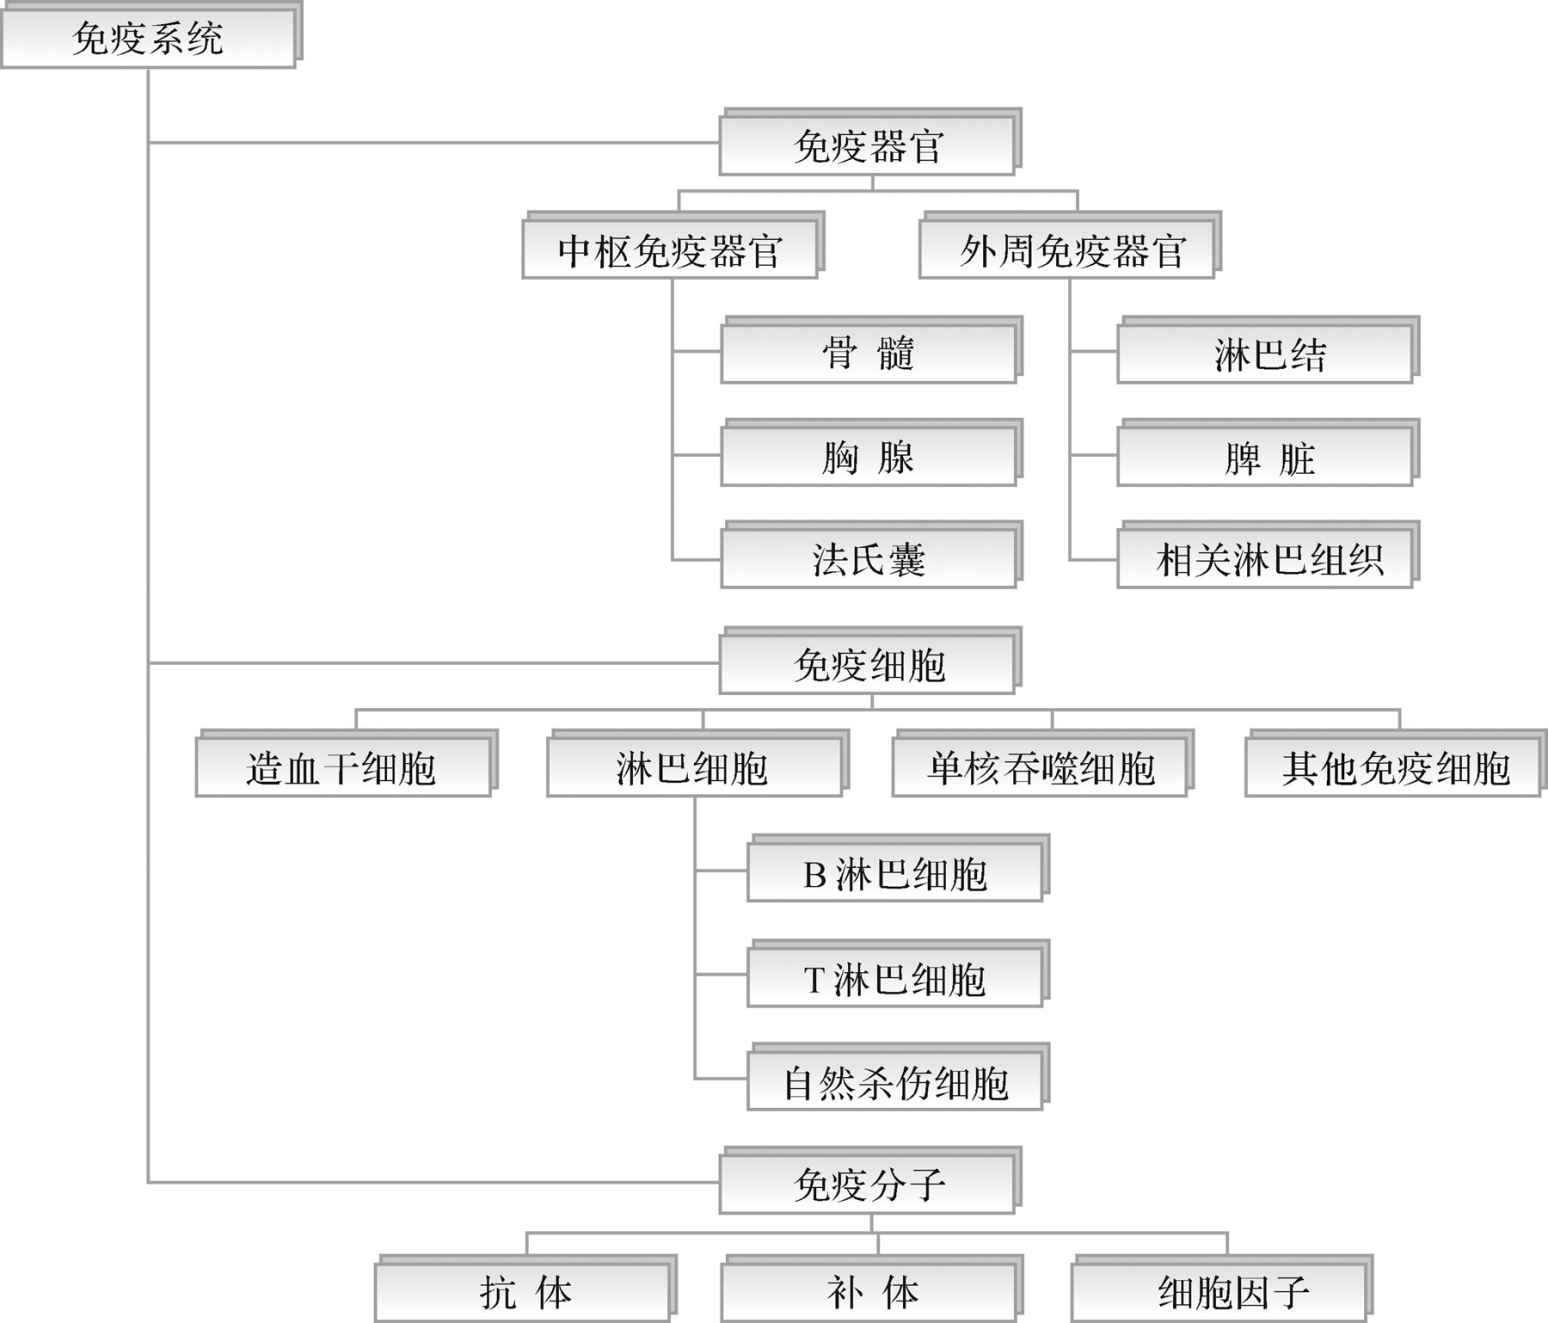
\includegraphics[width=.66\textwidth]{./images/Image00025.jpg}
\end{center}

\noindent\textbf{【课前思考】}

与机体的其他组织系统一样,免疫系统由哪些组织、器官、细胞组成?各种器官、细胞有何特征?在维护我们机体健康中各自起到怎样的作用?当有病原微生物入侵时,机体的各种免疫细胞是怎样各司其职又相互协调的?机体的免疫系统与国家的防御体系有何相似之处?

\noindent\textbf{【本章重点】}

1.免疫系统的构成;

2.免疫器官、免疫细胞的功能。

\noindent\textbf{【教学目标】}

1.掌握免疫系统组成:免疫器官(中枢免疫器官、外周免疫器官)、免疫细胞、免疫分子;

2.掌握中枢免疫器官的组成:骨髓、胸腺的主要免疫功能;

3.掌握外周免疫器官与组织的组成:淋巴结、脾脏的主要免疫功能。
\end{framed}
机体抵御外界病原微生物的入侵有三道防卫系统:

1.皮肤、黏膜及其分泌物

皮肤黏膜的机械阻挡作用和附属物(如纤毛)的清除作用,皮肤黏膜分泌物(如汗腺分泌的乳酸、胃黏膜分泌的胃酸等)的杀菌作用,体表和与外界相通的腔道中寄居的正常微生物丛对入侵微生物的拮抗作用等,属于机体第一道防线。其次是内部屏障。抗原物质一旦突破第一道防线进入机体后,即遭到机体内部屏障的清除,包括:淋巴和单核吞噬细胞系统屏障、正常体液中的一些非特异性杀菌物质、血脑屏障和胎盘屏障等(图\ref{fig2-1})。

\begin{figure}[!htbp]
 \centering
 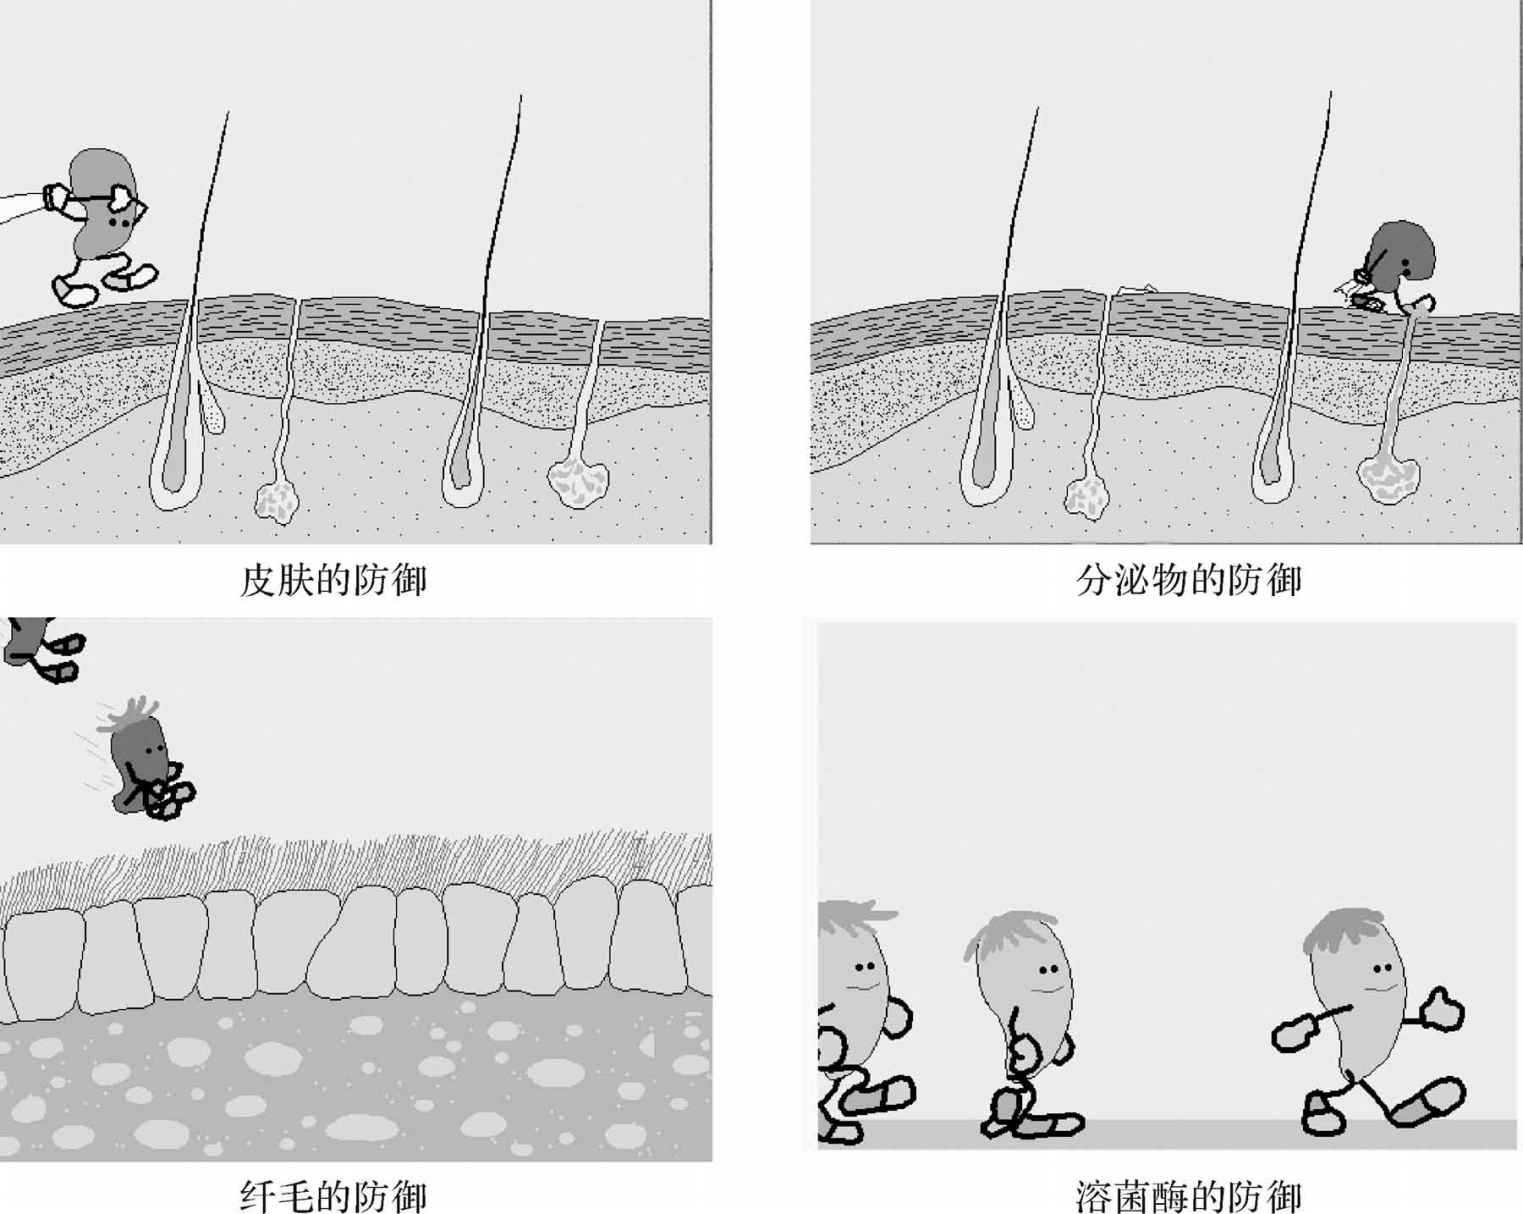
\includegraphics[width=.6\textwidth]{./images/Image00026.jpg}
 \caption{机体第一道防线}
 \label{fig2-1}
  \end{figure} 

2.吞噬细胞、NK细胞、抗菌蛋白、炎症应答------淋巴系统

微生物进入机体组织以后,多数沿组织细胞间隙的淋巴液经淋巴管到达淋巴结,但淋巴结内的巨噬细胞会消灭它们,阻止它们在机体内扩散,这就是淋巴屏障作用。如果微生物数量大、毒力强,就有可能冲破淋巴屏障,进入血液循环,扩散到组织器官中去。这时,它们会受到单核吞噬细胞系统屏障的阻挡。这是一类大的吞噬细胞。机体内还有一类较小的吞噬细胞,其中主要的是中性粒细胞和嗜酸性粒细胞。它们不属于单核吞噬细胞系统,但与单核吞噬细胞系统一样,分布于全身,对入侵的微生物和大分子物质有吞噬、消化和消除的作用。

在正常体液中的一些非特异性杀菌物质,如补体、调理素、溶菌酶、干扰素、乙型溶素、吞噬细胞杀菌素等,也与淋巴和单核吞噬细胞系统屏障一样,是机体的第二道防线,有助于消灭入侵的微生物(图\ref{fig2-2})。

\begin{figure}[!htbp]
 \centering
 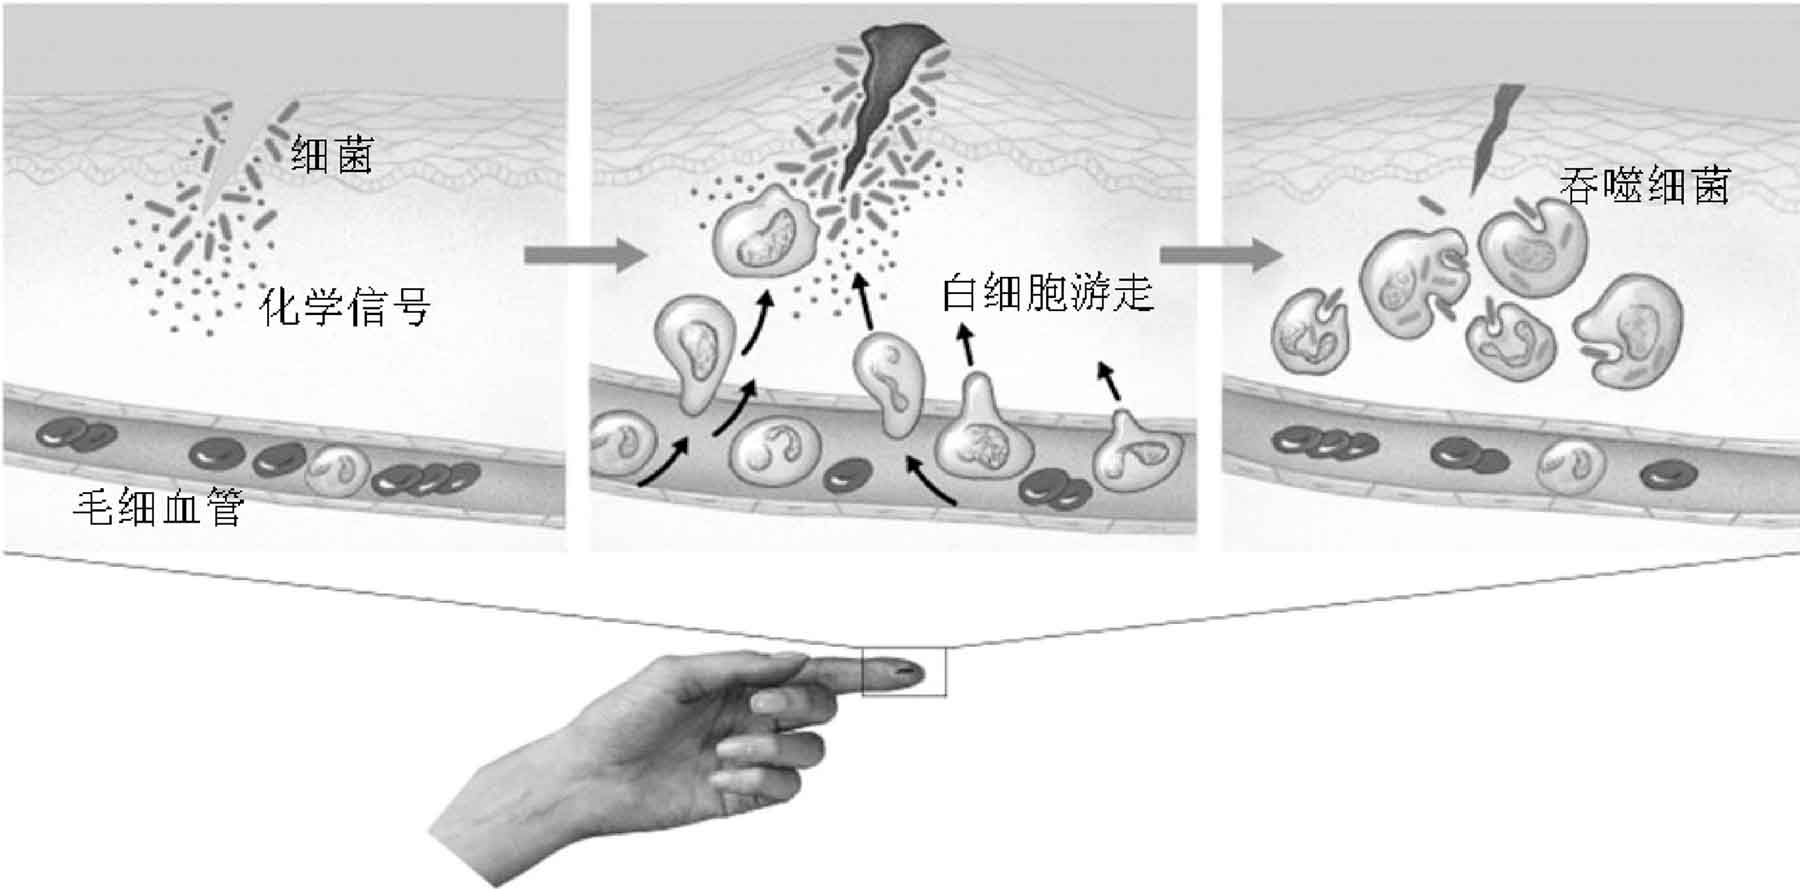
\includegraphics[width=.6\textwidth]{./images/Image00027.jpg}
 \caption{机体的第二道防线}
 \label{fig2-2}
  \end{figure} 

3.免疫系统:淋巴细胞、抗体;特点:特异性、多样性、记忆性、识别自我与非我(图\ref{fig2-3})。

\begin{figure}[!htbp]
 \centering
 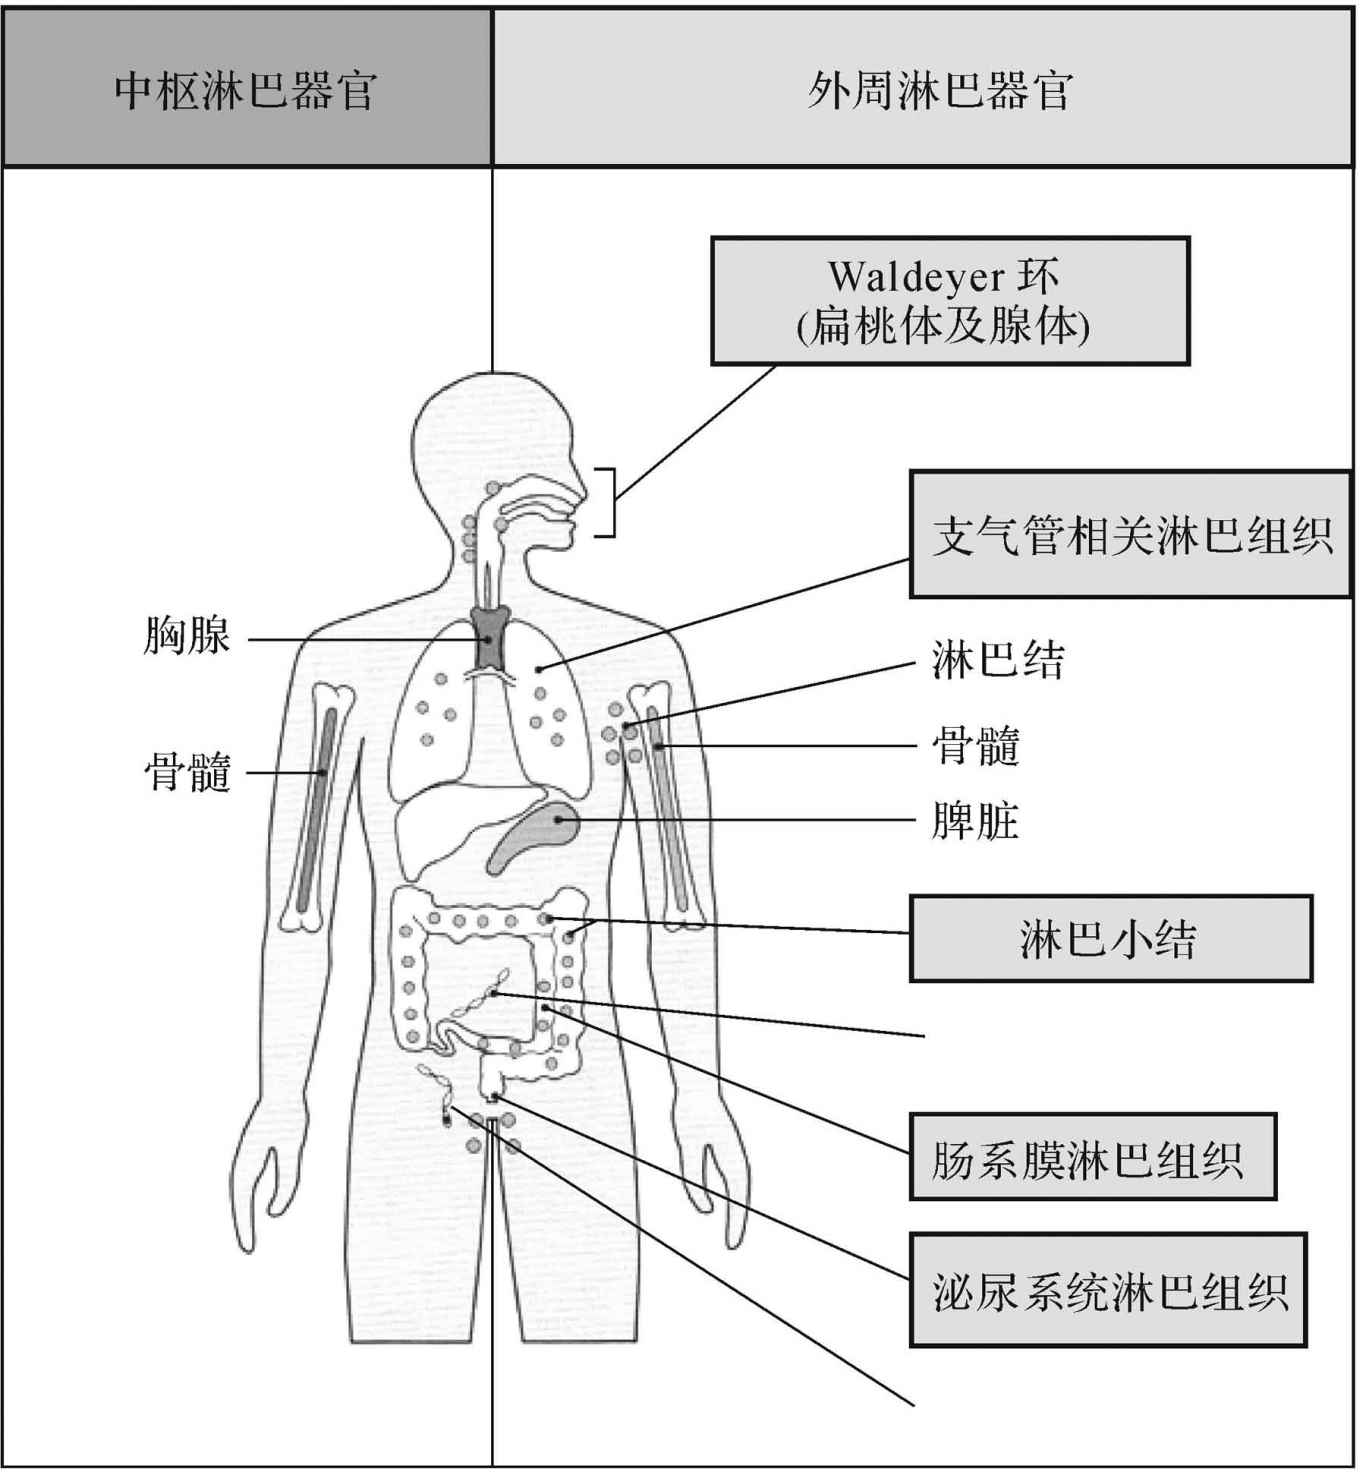
\includegraphics[width=.5\textwidth]{./images/Image00028.jpg}
 \caption{机体的第三道防线------免疫系统}
 \label{fig2-3}
  \end{figure} 

我们主要讲授免疫系统。

免疫系统(immune
system)乃承担免疫功能的组织系统,是机体对抗原刺激产生应答、执行免疫效应的物质基础。从宏观至微观进行描述,免疫系统包括免疫器官(中枢免疫器官和外周免疫器官)、免疫细胞(造血干细胞、淋巴细胞、单核吞噬细胞及其他免疫细胞)和免疫分子(抗体、补体、细胞因子)。

\section{中枢免疫器官}

中枢免疫器官(central immune
organ)是免疫细胞发生、分化、发育、成熟的场所,并对外周免疫器官的发育起主导作用,某些情况下(如再次抗原刺激或自身抗原刺激)也是产生免疫应答的场所。人和其他哺乳类动物的中枢免疫器官包括骨髓、胸腺,鸟类腔上囊(法氏囊)的功能相当于骨髓。


\subsection{骨髓}

骨髓(bone
marrow)是重要的中枢免疫器官,可分为红骨髓和白骨髓。红骨髓由结缔组织、血管、神经和实质细胞组成,呈海绵样存在于骨松质的腔隙中,具有活跃的造血功能。骨髓功能的发挥与其微环境有密切关系。骨髓微环境指造血细胞周围的微血管系统、末梢神经、网状细胞、基质细胞以及它们所表达的表面分子和所分泌的细胞因子。这些微环境组分是介导造血干细胞黏附、分化发育、参与淋巴细胞迁移和成熟的必需条件。骨髓是人和哺乳动物的造血器官(图\ref{fig2-4})。它具有如下功能:

1.各类免疫细胞发生的场所:骨髓造血干细胞具有分化成不同血细胞的能力,故被称为多能造血干细胞(multiple
hematopoietic stem
cell,HSC)。在骨髓微环境中,HSC首先分化为髓样前体细胞(myeloid
progenitor)和淋巴样前体细胞(lymphoid
progenitor)。髓样前体细胞最终分化成为粒细胞、单核细胞、红细胞、血小板;淋巴样前体细胞分化为T淋巴细胞(简称T细胞)、B淋巴细胞(简称B细胞)和自然杀伤细胞(NK细胞)。

\begin{figure}[!htbp]
 \centering
 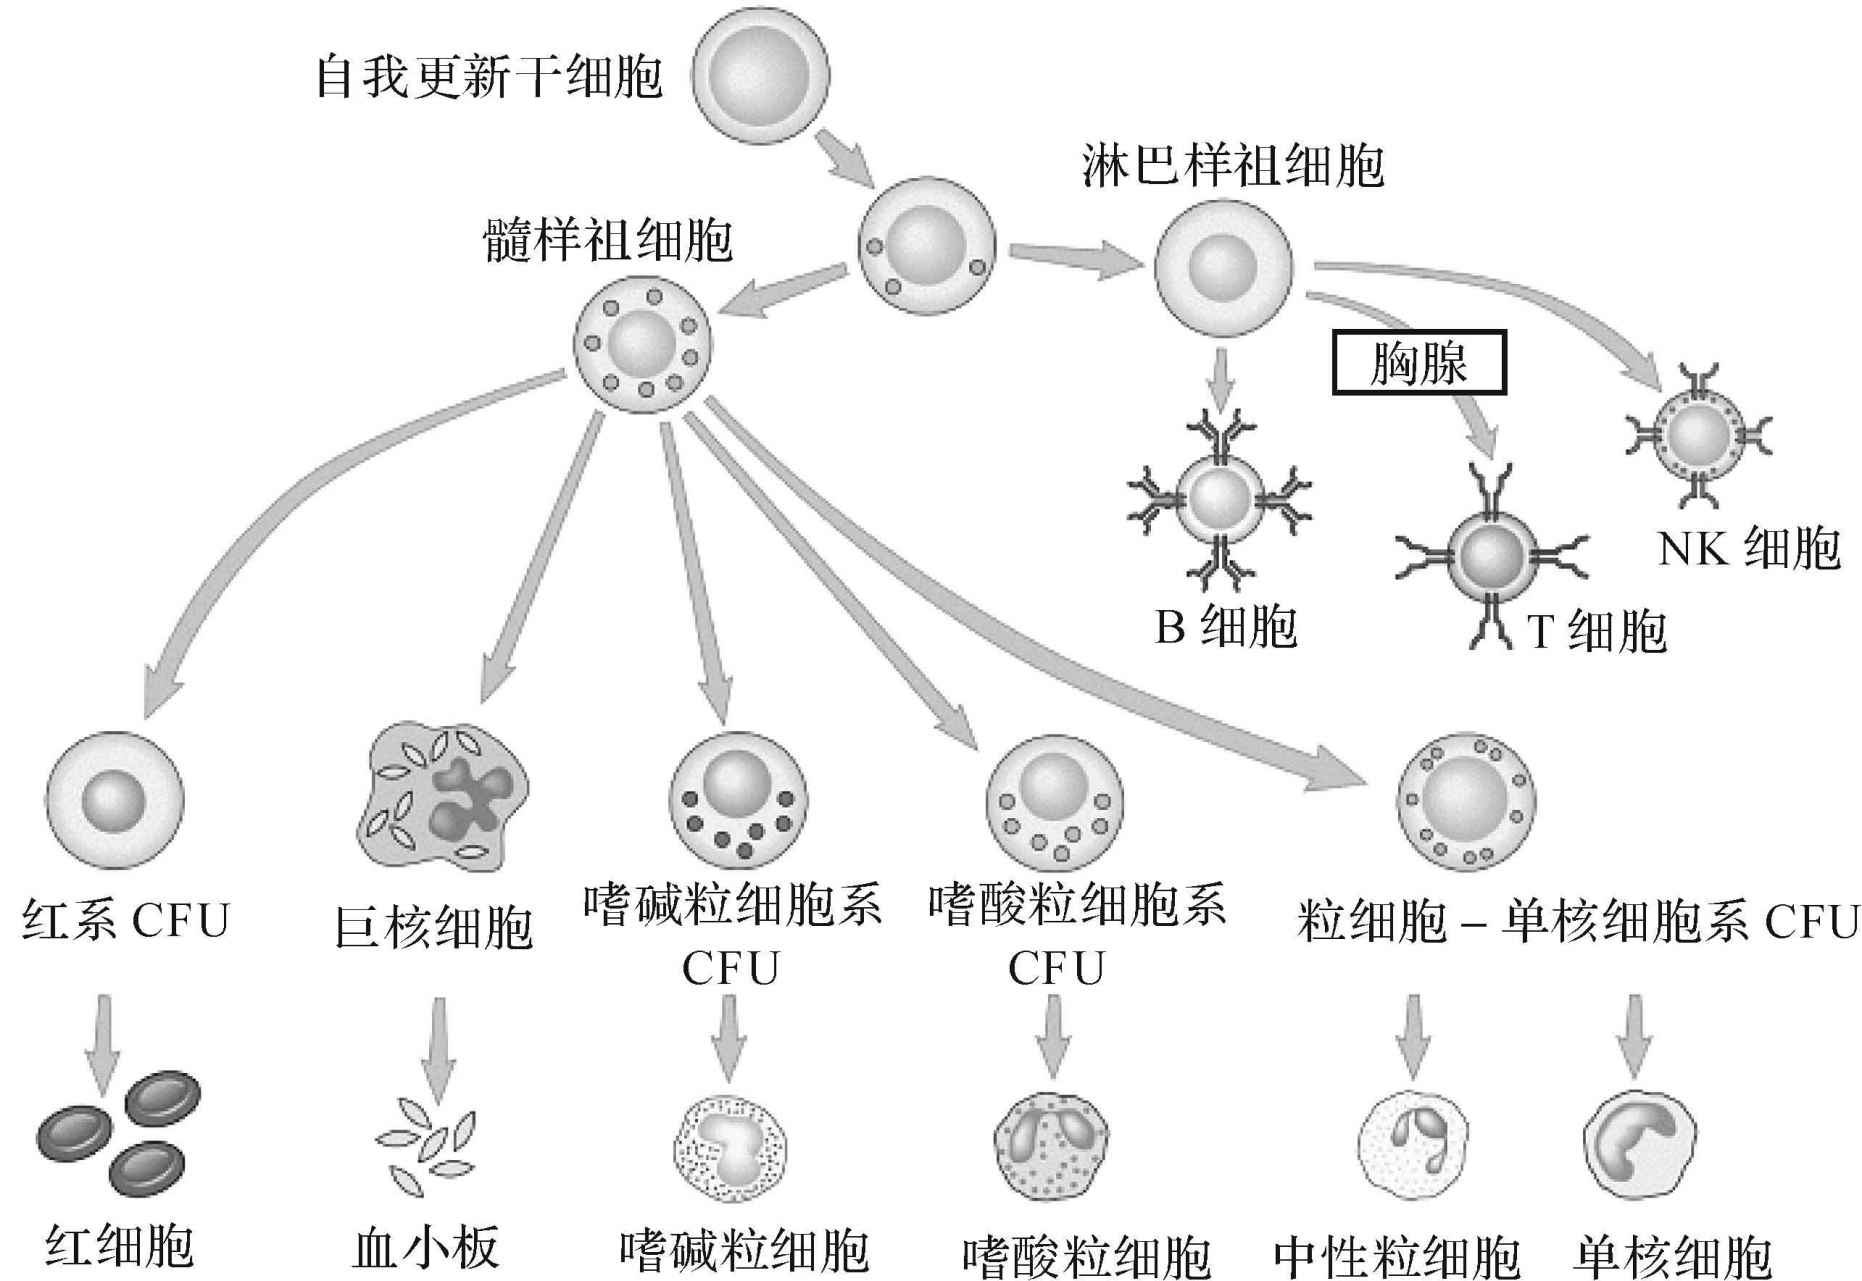
\includegraphics[width=.6\textwidth]{./images/Image00029.jpg}
 \caption{血细胞发育示意图}
 \label{fig2-4}
  \end{figure} 

2.B细胞分化成熟的场所:骨髓中产生的淋巴样前体细胞循不同的途径分化发育:一部分经血液迁入胸腺,发育成熟为成熟的T细胞;另一部分则在骨髓内继续分化为成熟B细胞。与T细胞在胸腺中分化的过程类似,B细胞在骨髓中也发生抗原受体(B
cell
receptor,BCR)等表面标志的表达、选择性发育或凋亡等。成熟的B细胞进入血循环,最终也定居在外周免疫器官。

3.发生B细胞应答的场所:骨髓是发生再次体液免疫应答的主要部位,外周免疫器官中的记忆性B细胞在抗原刺激下被活化,经淋巴液和血液进入骨髓后分化成熟为浆细胞,并产生大量抗体释放至血液循环。外周免疫器官中所发生的再次应答,其产生抗体的速度快,但持续时间短;而骨髓中所发生的再次应答,其产生抗体的速度慢,但可缓慢、持久地产生大量抗体,从而成为血清抗体的主要来源。

最新研究成果表明:在一定的微环境中,骨髓中的造血干细胞和基质干细胞还可分化为其他组织的多能干细胞(如神经干细胞、心肌干细胞等),这一突破性的进展开拓了骨髓生物学作用的全新领域,并可望在组织工程和临床医学中得到广泛应用。


\subsection{胸腺}

\begin{figure}[!htbp]
 \centering
 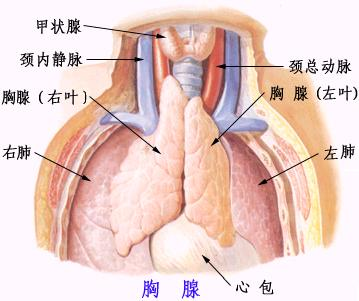
\includegraphics[width=0.5\textwidth]{./images/Image00030.jpg}
 \caption{人的胸腺}
 \label{fig2-5}
  \end{figure} 

人的胸腺(thymus)随年龄不同而有明显差别(图\ref{fig2-5})。新生期胸腺重量约15~20g;以后逐渐增大,青春期可达30~40g,其后随年龄增长而逐渐萎缩退化;老年期胸腺明显缩小,大部分被脂肪组织所取代。胸腺是T细胞分化、成熟的场所,其功能状态直接决定机体细胞免疫功能,并间接影响体液免疫功能。

(一)胸腺的解剖结构

胸腺的结构如图\ref{fig2-6}所示。一结缔组织被膜覆盖胸腺表面,并深入胸腺实质将其分隔成许多小叶。小叶的外层为皮质(cortex),内层为髓质(medulla),皮髓质交界处含大量血管,皮质内85\%~90\%的细胞为未成熟T细胞(即胸腺细胞),也存在少量上皮细胞、巨噬细胞(macrophage,Mφ)和树突状细胞(dendritic
cell,DC)等。胸腺浅皮质内发育早期的胸腺上皮细胞也称抚育细胞(nurse
cell),其在胸腺细胞分化中发挥重要作用。髓质内含大量上皮细胞和疏散分布的胸腺细胞、Mφ和DC。

\begin{figure}[!htbp]
 \centering
 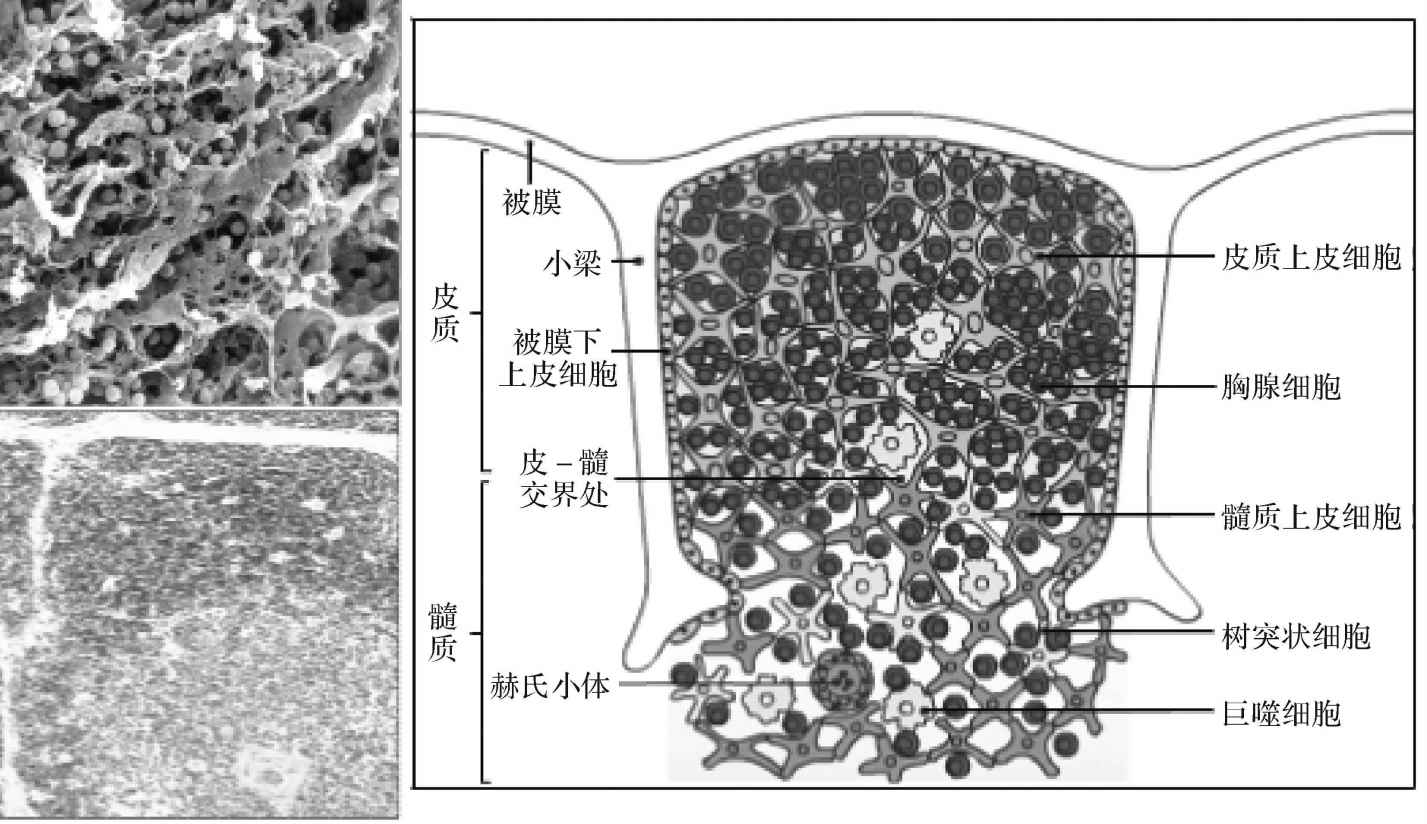
\includegraphics[width=0.7\textwidth]{./images/Image00031.jpg}
 \caption{胸腺结构示意图}
 \label{fig2-6}
  \end{figure} 

(二)胸腺的细胞组成:主要由胸腺基质细胞和胸腺细胞组成

1.胸腺基质细胞(thymic stromal cell,TSC):TSC以胸腺上皮细胞(thymus
epithelial
cell,TEC)为主,还包括巨噬细胞、DC及成纤维细胞等。TSC互相连接成网,并表达多种表面分子和分泌多种胸腺激素,从而构成重要的胸腺内环境。其中,抚育细胞与胸腺细胞通过各自表达的黏附分子密切接触,为胸腺细胞的发育提供必需的信号。

2.胸腺细胞:骨髓产生的前T细胞经血循环进入胸腺,即成为胸腺细胞。不同分化阶段的胸腺细胞其形态学、表面标志等各异,并可按其CD4、CD8表达情况分为4个亚群,即:CD4\textsuperscript{-}
CD8\textsuperscript{-} 、CD4\textsuperscript{+} CD8\textsuperscript{+}
、CD4\textsuperscript{+} CD8\textsuperscript{-} 、CD4\textsuperscript{-}
CD8\textsuperscript{+} 。

(三)胸腺微环境

胸腺微环境由TSC、细胞外基质及局部活性物质组成,其在胸腺细胞分化过程的不同环节均发挥重要作用。胸腺上皮细胞是胸腺微环境的最重要组分,其参与胸腺细胞分化的机制为:

1.分泌胸腺激素和细胞因子:主要的胸腺激素有胸腺素(thymosin)、胸腺刺激素(thymulin)、胸腺体液因子(thymic
humoral factor)、胸腺生成素(thymopoietin,TP)、血清胸腺因子(serum
thymic
factor)等。它们分别具有促进胸腺细胞增殖和分化、发育等功能。胸腺基质细胞还可产生多种细胞因子,它们通过与胸腺细胞表面相应受体结合,调节胸腺细胞发育和细胞间相互作用。上述胸腺激素和细胞因子是诱导胸腺细胞分化为成熟T细胞的必要条件。

2.与胸腺细胞相互接触:此乃通过上皮细胞与胸腺细胞间表面黏附分子及其配体、细胞因子及其受体、抗原肽-MHC分子复合物与TCR等相互作用而实现。

细胞外基质(extracellular
matrix)也是胸腺微环境的重要组成部分,它们可促进上皮细胞与胸腺细胞接触,并参与胸腺细胞在胸腺内移行成熟。

(四)胸腺的功能

1.T细胞分化、成熟的场所:胸腺是T细胞发育的主要场所。在胸腺产生的某些细胞因子作用下,来源于骨髓的前T细胞被吸引至胸腺内成为胸腺细胞。胸腺细胞循被膜下转移到皮质再向髓质移行,并经历十分复杂的选择性发育。在此过程中,约95\%的胸腺细胞发生以凋亡(apoptosis)为主的死亡而被淘汰,仅不足5\%的细胞分化为成熟T细胞。其特征为:表达成熟抗原受体(TCR)的CD4或CD8单阳性细胞;获得MHC限制性的抗原识别能力;获得自身耐受性。发育成熟的T细胞进入血循环,最终定居于外周免疫器官。

近期研究证实,胸腺并非T细胞分化发育的唯一场所。例如T细胞可在胸腺外组织(如肠道黏膜上皮、皮肤组织及泌尿生殖道黏膜组织等)中发育成熟。另外,肝脏也可能是某些T细胞分化发育的场所。

2.免疫调节功能:胸腺基质细胞可产生多种肽类激素,它们不仅促进胸腺细胞的分化成熟,也参与调节外周成熟T细胞。

3.屏障作用:皮质内毛细血管及其周围结构具有屏障作用,阻止血液中大分子物质进入,此为血-胸腺屏障(blood-thymus
barrier)。


\subsection{腔上囊}

腔上囊又称法氏囊(bursa of
fabricius),是鸟类动物特有的淋巴器官,位于胃肠道末端泄殖腔的后上方(图\ref{fig2-7})。与胸腺不同,腔上囊训化B细胞成熟,主导机体的体液免疫功能。将孵出的雏鸡去掉腔上囊,会使血中γ球蛋白缺乏,且没有浆细胞,注射疫苗亦不能产生抗体。人类和哺乳动物没有法氏囊,其功能由相似的组织器官代替,称为法氏囊同功器官;曾一度认为同功器官是阑尾、扁桃体和肠集结淋巴结,现在已证明是骨髓。

\begin{figure}[!htbp]
 \centering
 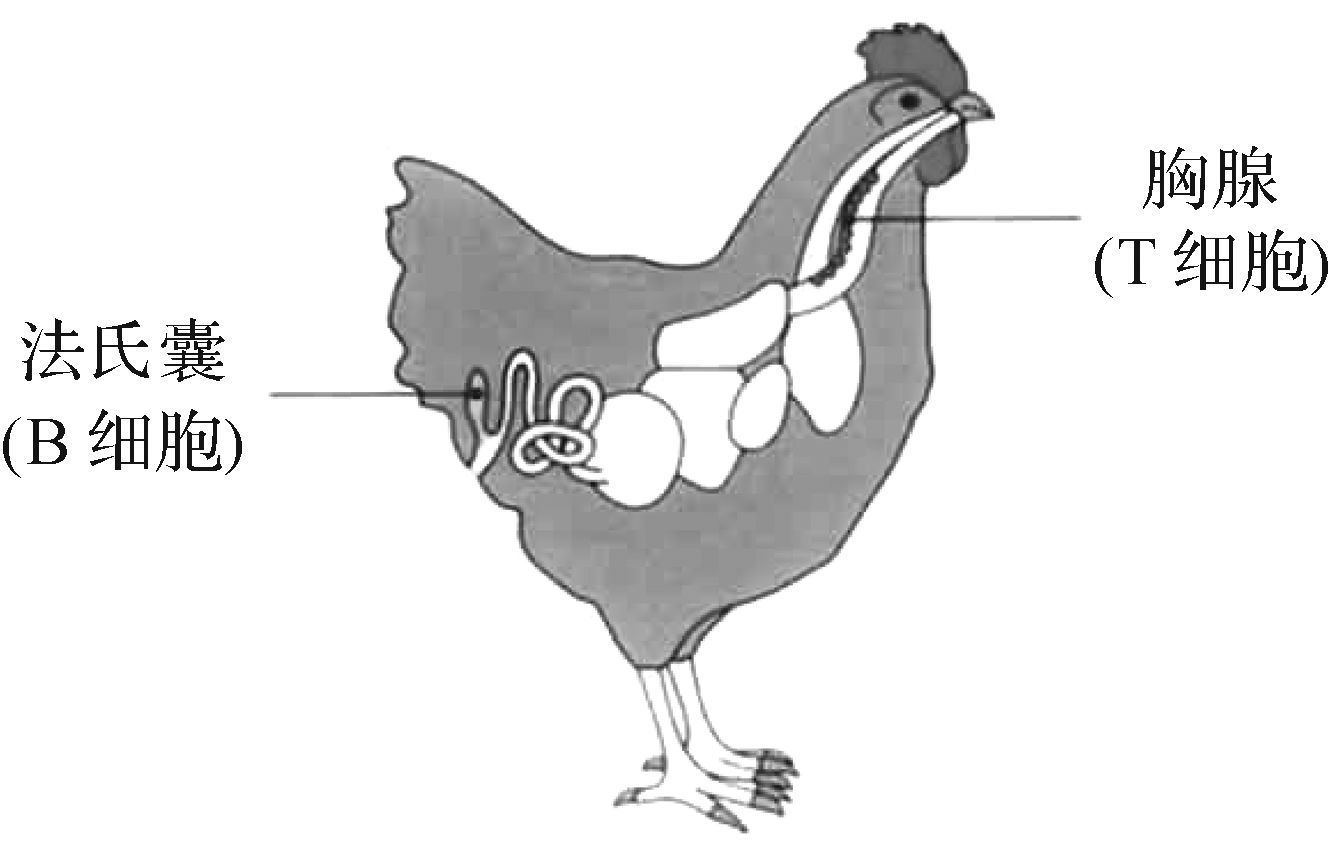
\includegraphics[width=.5\textwidth]{./images/Image00032.jpg}
 \caption{鸡的胸腺和法氏囊}
 \label{fig2-7}
  \end{figure} 

\section{外周免疫器官}

外周免疫器官(peripheral immune
organ)包括脾、淋巴结、淋巴样小结、扁桃体、阑尾等,这些器官内富含能捕捉和处理抗原的巨噬细胞和树突状细胞,以及能介导免疫反应的T细胞和B细胞。


\subsection{淋巴结}

淋巴结(lymph node)广泛分布于全身非黏膜部位的淋巴通道上。

(一)淋巴结的结构

淋巴结的结构如图\ref{fig2-8}所示,淋巴结表面覆盖有结缔组织被膜,后者深入实质形成小梁。淋巴结分为皮质和髓质两部分,彼此通过淋巴窦相通。被膜下为皮质,包括浅皮质区、副皮质区和皮质淋巴窦。

浅皮质区又称为非胸腺依赖区(thymus-independent
area),是B细胞定居的场所,该区内有淋巴滤泡(或称淋巴小结)。未受抗原刺激的淋巴小结无生发中心,称为初级滤泡(primary
follicle),主要含静止的成熟B细胞;受抗原刺激的淋巴小结内出现生发中心(germinal
center),称为次级滤泡(secondary
follicle),内含大量增殖分化的B淋巴母细胞,此细胞向内转移至淋巴结中心部髓质,即转化为可产生抗体的浆细胞。

副皮质区又称胸腺依赖区(thymus-dependent
area),位于浅皮质区和髓质之间,为深皮质区,是T细胞(主要是CD\textsuperscript{+}
\textsubscript{4}
T细胞)定居的场所。该区有许多由内皮细胞组成的毛细血管后微静脉,也称高内皮细胞小静脉(high
endothelial venule,HEV),在淋巴细胞再循环中起重要作用。

髓质由髓索和髓窦组成。髓索内含有
B细胞、T细胞、浆细胞、肥大细胞及Mφ。髓窦内Mφ较多,有较强滤过作用。

\begin{figure}[!htbp]
 \centering
 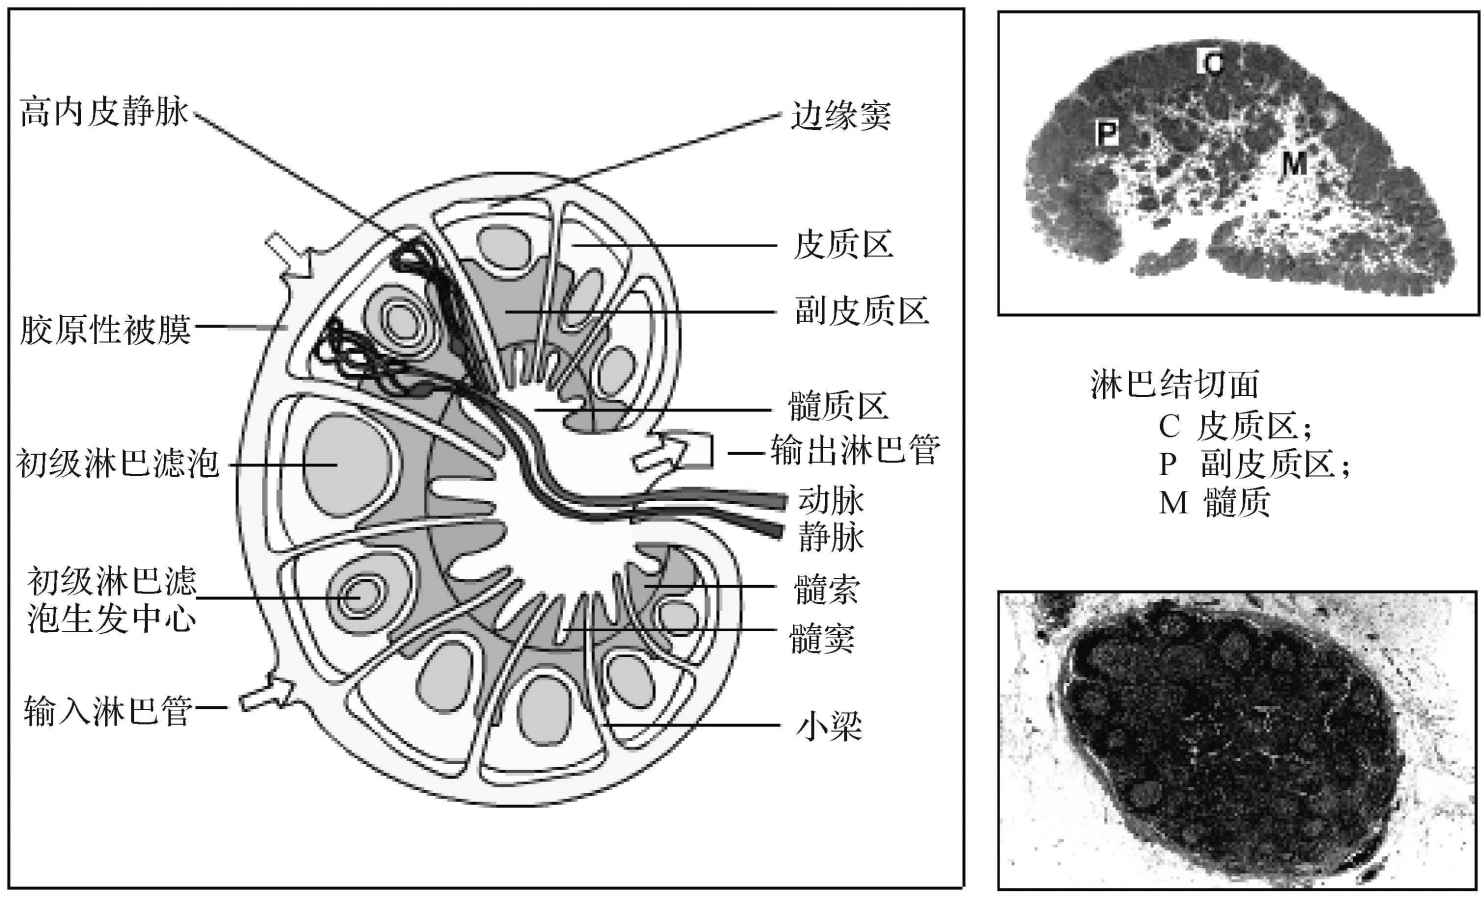
\includegraphics[width=.6\textwidth]{./images/Image00033.jpg}
 \caption{淋巴结的结构}
 \label{fig2-8}
  \end{figure} 

(二)淋巴结的功能

1.T 细胞及
B细胞定居的场所:分别在胸腺和骨髓中分化成熟的T、B细胞,均可定居于淋巴结。其中,T细胞占淋巴结内淋巴细胞总数的75\%,B细胞占25\%。

2.免疫应答发生的场所:抗原递呈细胞携带所摄取的抗原进入淋巴结,将已被加工、处理的抗原递呈给淋巴结内的T细胞和B细胞,使之活化、增殖、分化,故淋巴结是发生细胞免疫和体液免疫应答的主要场所。

3.参与淋巴细胞再循环:淋巴结深皮质区的HEV在淋巴细胞再循环中发挥重要作用,血循环中的淋巴细胞穿越HEV壁进入淋巴结实质,然后通过输出淋巴管进入胸导管或右淋巴管,再回到血液循环。

4.过滤作用:组织中的病原微生物及毒素等进入淋巴液,其缓慢流经淋巴结时,可被Mφ吞噬或通过其他机制被清除。因此,淋巴结具有重要的滤过作用。


\subsection{脾脏}

(一)脾脏的结构

脾脏的结构如图\ref{fig2-9}所示,脾脏(spleen)是人体最大的淋巴器官,可分为白髓、红髓和边缘区三部分。白髓由密集的淋巴组织构成,包括动脉周围淋巴鞘和淋巴小结。动脉周围淋巴鞘为T细胞居住区;鞘内的淋巴小结为B细胞居住区,未受抗原刺激为初级滤泡,受抗原刺激后出现生发中心,为次级滤泡。红髓分布于白髓周围,包括髓索和髓窦:前者主要为B细胞居留区,也含Mφ和DC;髓窦内为循环的血液。白髓与红髓交界处为边缘区(marginal
zone),是血液及淋巴细胞进出的重要通道。

\begin{figure}[!htbp]
 \centering
 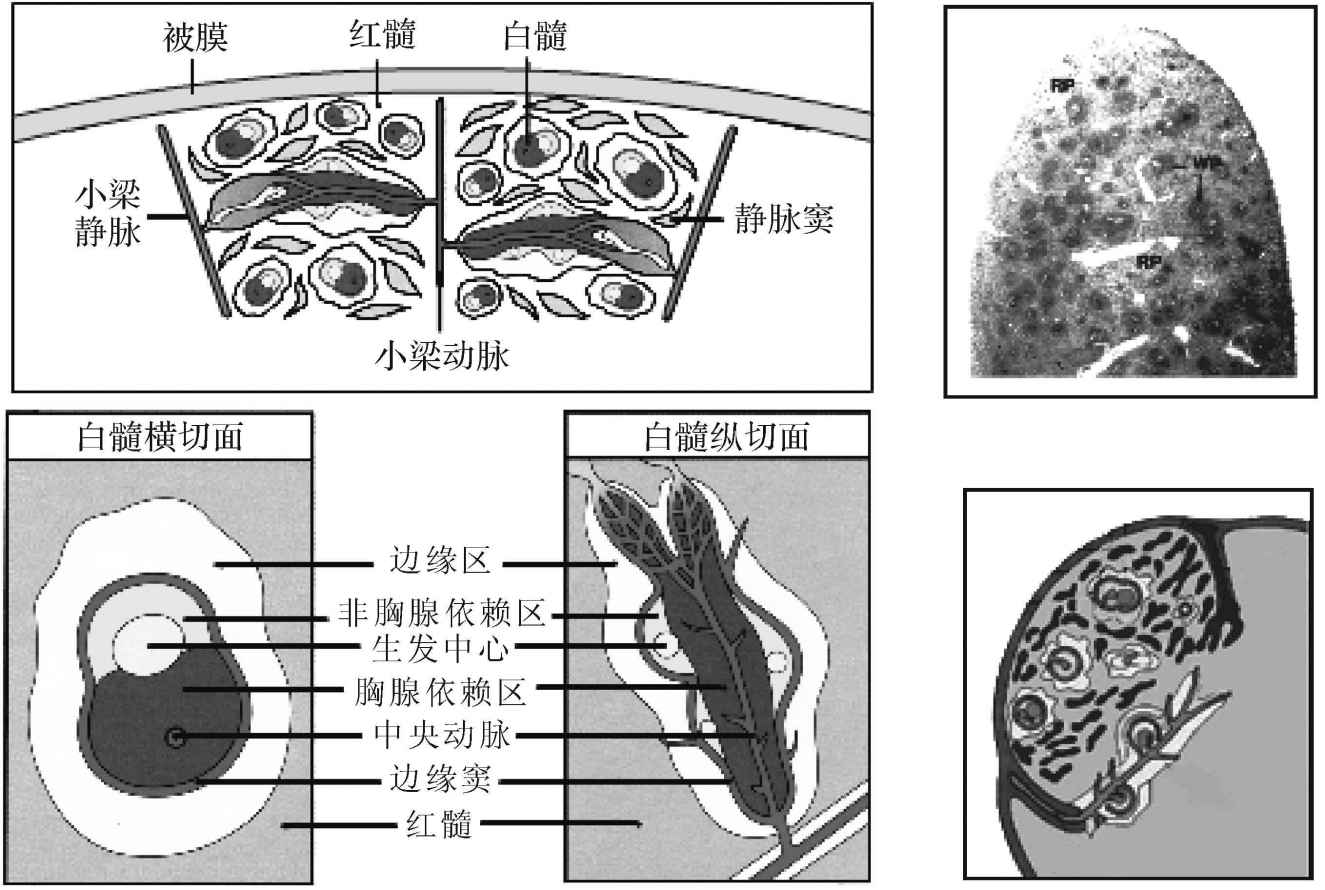
\includegraphics[width=.5\textwidth]{./images/Image00034.jpg}
 \caption{脾脏的结构}
 \label{fig2-9}
  \end{figure} 

(二)脾脏的功能

脾脏是重要的外周免疫器官,脾切除的个体其免疫防御功能可发生障碍。

1.免疫细胞定居的场所:成熟的淋巴细胞可定居于脾脏。B细胞约占脾脏中淋巴细胞总数的60\%,T细胞约占40\%。

2.免疫应答的场所:脾脏也是淋巴细胞接受抗原刺激并发生免疫应答的重要部位。同为外周免疫器官,脾脏与淋巴结的差别在于:脾脏是对血源性抗原产生应答的主要场所。

3.合成生物活性物质:脾脏可合成并分泌如补体、干扰素等生物活性物质。

4.滤过作用:脾脏可清除血液中的病原体、衰老死亡的自身血细胞、某些蜕变细胞及免疫复合物等,从而使血液得到净化。

此外,脾脏也是机体贮存红细胞的血库。


\subsection{黏膜相关淋巴组织}

黏膜相关淋巴组织(mucosal-associated lymphoid
tissue,MALT)亦称黏膜免疫系统(mucosal lymphoid
system,MIS),主要指呼吸道、肠道及泌尿生殖道黏膜固有层和上皮细胞下散在的无被膜淋巴组织以及某些带有生发中心的器官化淋巴组织,如扁桃体、小肠的派氏集合淋巴结(Peyer
patche)、阑尾等。

黏膜系统在机体免疫防疫机制中的重要作用表现为:①人体黏膜的表面积约400平方米,乃阻止病原微生物等入侵机体的主要物理屏障;②机体近一半的淋巴组织存在于黏膜系统,故MALT被视为执行局部特异性免疫功能的主要部位。

(一)MALT的组成

1.鼻相关淋巴组织(nasal-associated lymphoid
tissue,NALT):包括咽扁桃体、腭扁桃体、舌扁桃体及鼻后部其他淋巴组织,其主要作用是抵御经空气传播的微生物感染。

2.肠相关淋巴组织(gut-associated lymphoid
tissue,GALT):GALT包括集合淋巴结、淋巴滤泡和固有层淋巴组织等,其主要作用是抵御侵入肠道的病原微生物感染(图\ref{fig2-10})。肠道黏膜上皮间还散布一种扁平上皮细胞,即M细胞(membranous
cell or microfold
cell,膜性细胞或微皱褶细胞),又称特化的抗原转运细胞(specialized
antigen transporting
cell),是散布于肠道黏膜上皮细胞间的一种特化的抗原运转细胞。它不表达MHCⅡ类分子,胞质内溶毛体很少,在肠黏膜表面有短小不规则毛刷样微绒毛。M细胞的基底部凹陷成小袋,其中容纳T细胞、B细胞、巨噬细胞、DC等。M细胞具有高度的非特异性脂酶活性,病原菌等外来抗原性物质可通过对M细胞表面的毛刷状微绒毛的吸附,或经M细胞表面蛋白酶作用后被摄取,并将未降解的抗原转运给小袋中的巨噬细胞,由后者携带抗原至集合淋巴结,引发黏膜免疫应答,肠道淋巴系统免疫应答如图\ref{fig2-11}所示。

\begin{figure}[!htbp]
 \centering
 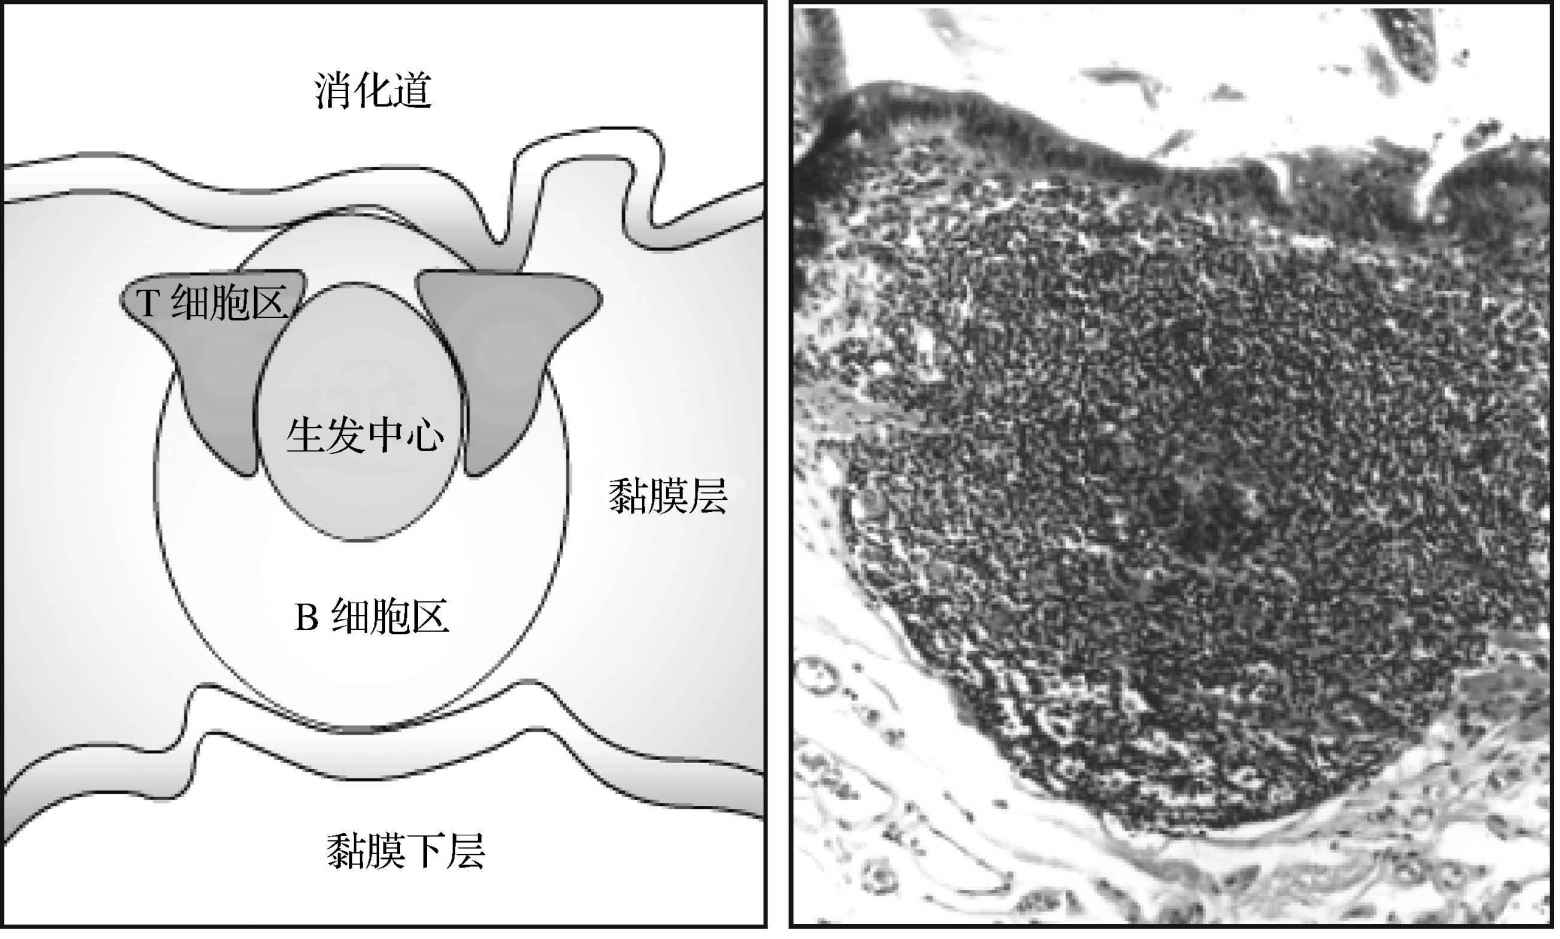
\includegraphics[width=.5\textwidth]{./images/Image00035.jpg}
 \caption{消化道集合淋巴滤泡}
 \label{fig2-10}
  \end{figure} 

\begin{figure}[!htbp]
 \centering
 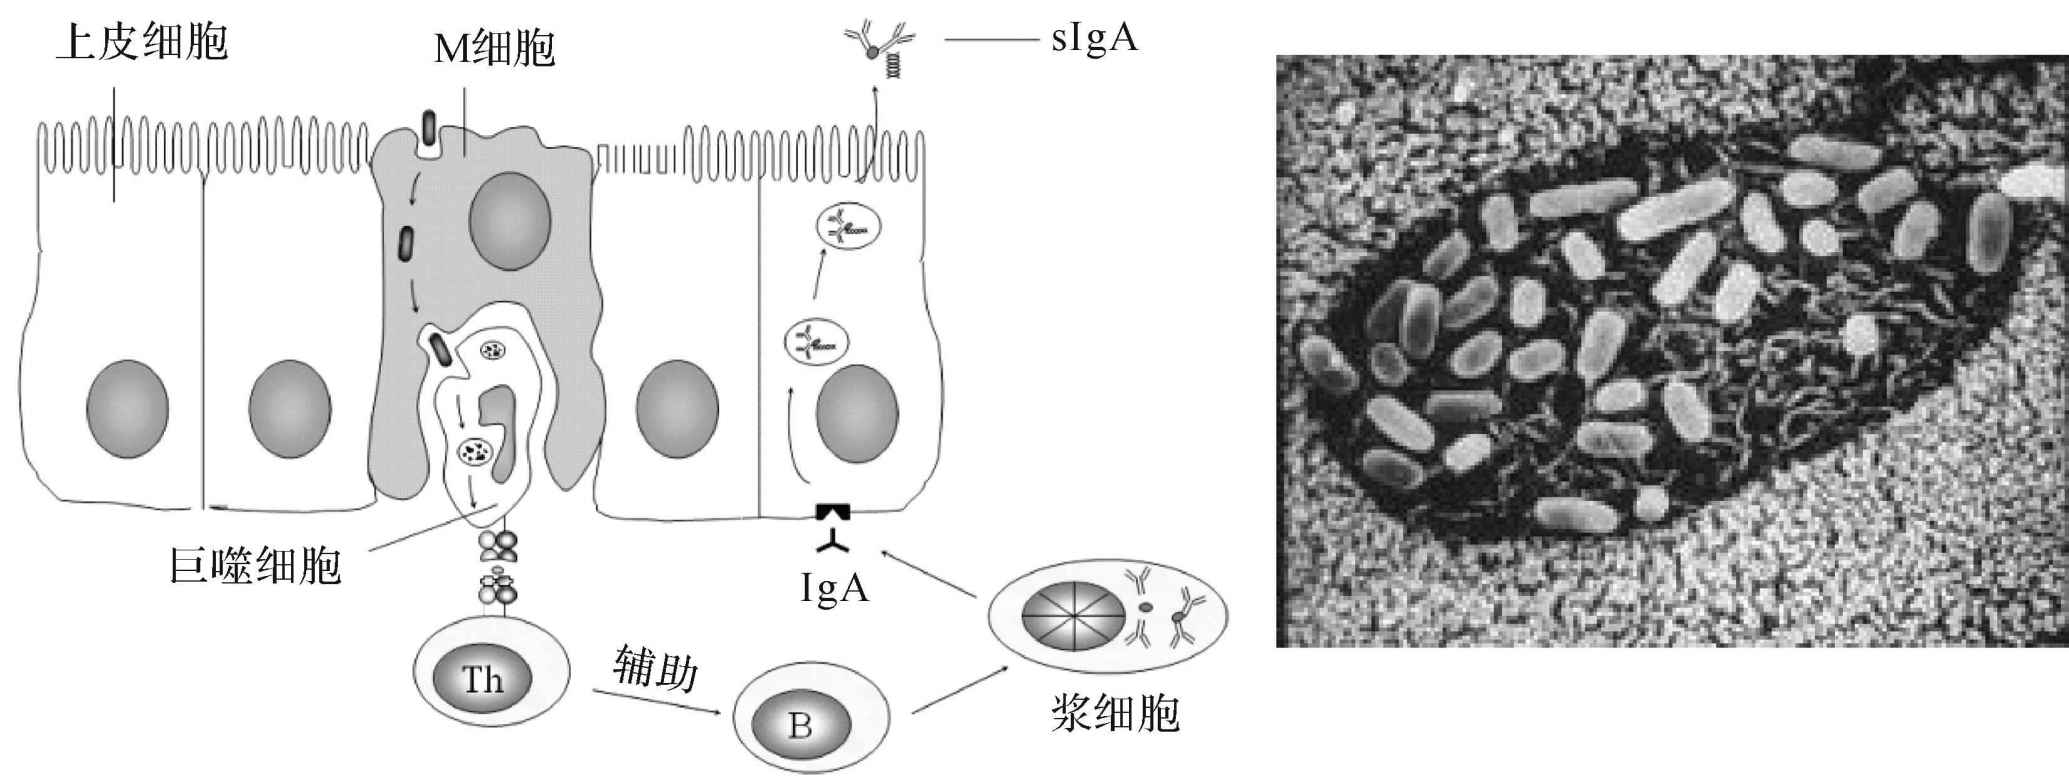
\includegraphics[width=.6\textwidth]{./images/Image00036.jpg}
 \caption{肠道M细胞的转运功能及M细胞包围住大肠杆菌}
 \label{fig2-11}
  \end{figure} 

黏膜免疫系统在保护黏膜表面不受病原体侵害、促进与共生微生物群落共生中都起主要作用。要激发黏膜免疫反应,黏膜表面上的抗原必须首先穿过不可透过的上皮障碍,进入“派伊尔小结”这样的淋巴结构。这一功能(被称为“转胞吞作用”)被认为主要由M细胞调控,它们是“派伊尔小结”中专门的上皮细胞。对由M-细胞调控的抗原“转胞吞作用”的机制所做的一项研究表明,在小肠M细胞顶面表达的糖蛋白-2是表达FimH抗原的细菌的转胞吞受体。由于M-细胞被认为是各种口服免疫药物的一个很有希望的目标,所以这项工作表明,依赖于糖蛋白-2的“转胞吞作用”是一个可能的免疫目标。

3.支气管相关淋巴组织(bronchial-associated
tissue,BALT):主要分布于各肺叶的支气管上皮下,其结构与派氏集合淋巴结相似,滤泡中淋巴细胞受抗原刺激常增生成生发中心,其中主要是B细胞。

(二)MALT的功能及其特点

1.参与局部免疫应答:分布在不同部位的MALT均是参与局部特异性免疫应答的主要场所,从而在消化道、呼吸道和泌尿生殖道的局部免疫防御中发挥关键作用。

2.分泌型IgA(secretory
IgA,SIgA):以消化道黏膜为例,口服抗原被吸收进入集合淋巴结后,可引发B细胞应答,使之转化为产生抗体的浆细胞,其中可分泌SIgA的浆细胞主要定居于集合淋巴结或迁移至固有层。SIgA在抵御病原体侵袭消化道、呼吸道和泌尿生殖道中发挥重要作用。

3.参与口服抗原介导的免疫耐受:口服蛋白抗原刺激黏膜免疫系统后,常可导致免疫耐受,其机制尚未阐明。口服抗原诱导耐受的生物学意义在于:①可阻止机体对肠腔内共栖的正常菌群产生免疫应答,而这些菌群的存在乃正常消化和吸收功能所必需;②通过口服抗原诱导机体对该抗原形成特异性无反应性,可能为治疗自身免疫病提供新途径。

\begin{center}
\textbf{\Large 附:淋巴细胞再循环}
\end{center}

各种免疫器官中的淋巴细胞并不是定居不动的群体,而是通过血液和淋巴液的循环进行有规律的迁移,这种规律性的迁移为淋巴细胞再循环(lymphocyterecirculation)。通过再循环,可以增加淋巴细胞与抗原接触的机会,更有效地激发免疫应答,并不断更新和补充循环池的淋巴细胞。

1.再循环的细胞淋巴干细胞从骨髓迁移至胸腺和腔上囊或其功能器官,分化成熟后进入血液循环的定向移动过程不属于再循环范围。再循环是成熟淋巴细胞通过循环途径实现淋巴细胞不断重新分布的过程。再循环中的细胞多是静止期细胞和记忆细胞,其中80%以上是T细胞。这些细胞最初来源于胸腺和骨髓;成年以后,主要靠外周免疫器官进行补充。受抗原刺激而活化的淋巴细胞很快定居于外周免疫器官,不再参加再循环。

2.再循环的途径血液中的淋巴细胞在流经外周免疫器官(以淋巴结为例)时,在副皮质区与皮质区的连接处穿过高内皮毛细血管后静脉(HEV)进入淋巴结;T细胞定位于副皮质,B细胞主要定位于皮质区;以后均通过淋巴结髓窦迁移至输出淋巴管,进入高一级淋巴结;经过类似的路径,所有外周免疫器官输出的细胞最后都汇集于淋巴导管;身体下部和左上部的汇集到胸导管,从左锁骨下静脉角返回血循环;右侧上部的汇集到右淋巴管,从右锁骨下静脉返回血循环。再循环一周约需24~48小时。

3.细胞定居选择淋巴细胞从血循环进入淋巴组织具有高度的选择性,这是因为淋巴细胞上具有特殊的受体分子,称为归巢受体(homingreceptor)。现已发现的归巢受体包括CD44、LFA-1、VLA-4和MEL-14/LAM-1等;其中MEL-14/LAM-1是定居淋巴结的受体,识别淋巴结内的高内皮细胞;VLA-4的α亚单位是定居MALT的受体,识别黏膜表面的配体。

淋巴细胞再循环的意义:带有不同特异性抗原受体的各种淋巴细胞不断在体内各处巡游,增加了与抗原以及抗原递呈细胞接触的机会;许多免疫记忆细胞也参与淋巴细胞再循环,一旦接触到相应抗原,可立即进入淋巴组织发生增殖反应,产生免疫应答。淋巴细胞再循环如图\ref{fig2-12}所示。

\begin{figure}[!htbp]
 \centering
 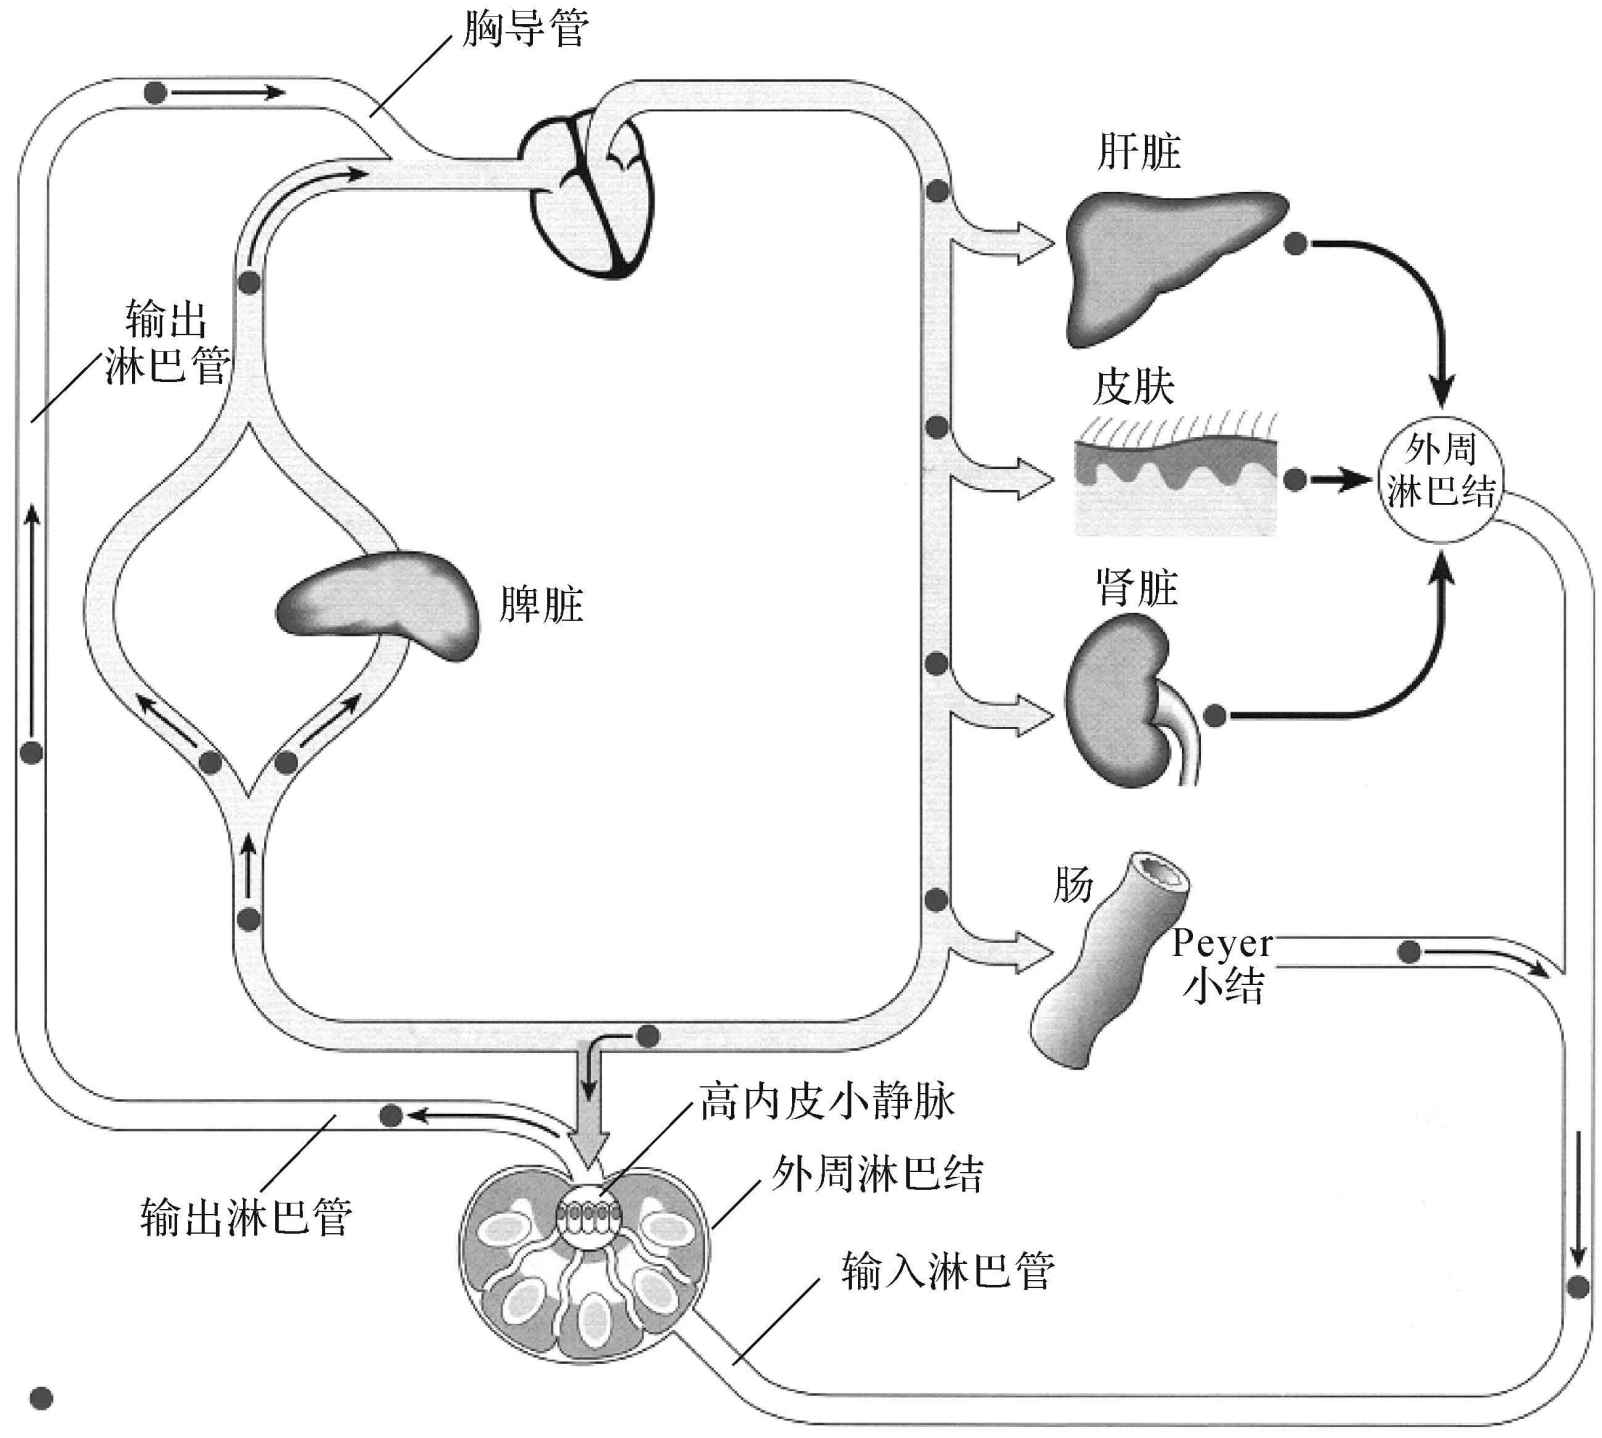
\includegraphics[width=.6\textwidth]{./images/Image00037.jpg}
 \caption{淋巴细胞再循环示意图}
 \label{fig2-12}
  \end{figure} 

\section{免疫细胞}

免疫细胞乃泛指所有参与免疫应答或与免疫应答有关的细胞及其前体,包括造血干细胞、淋巴细胞、专职抗原递呈细胞(树突状细胞、单核-巨噬细胞)及其他抗原递呈细胞、粒细胞、肥大细胞和红细胞等,如图\ref{fig2-13}所示。

\begin{figure}[!htbp]
 \centering
 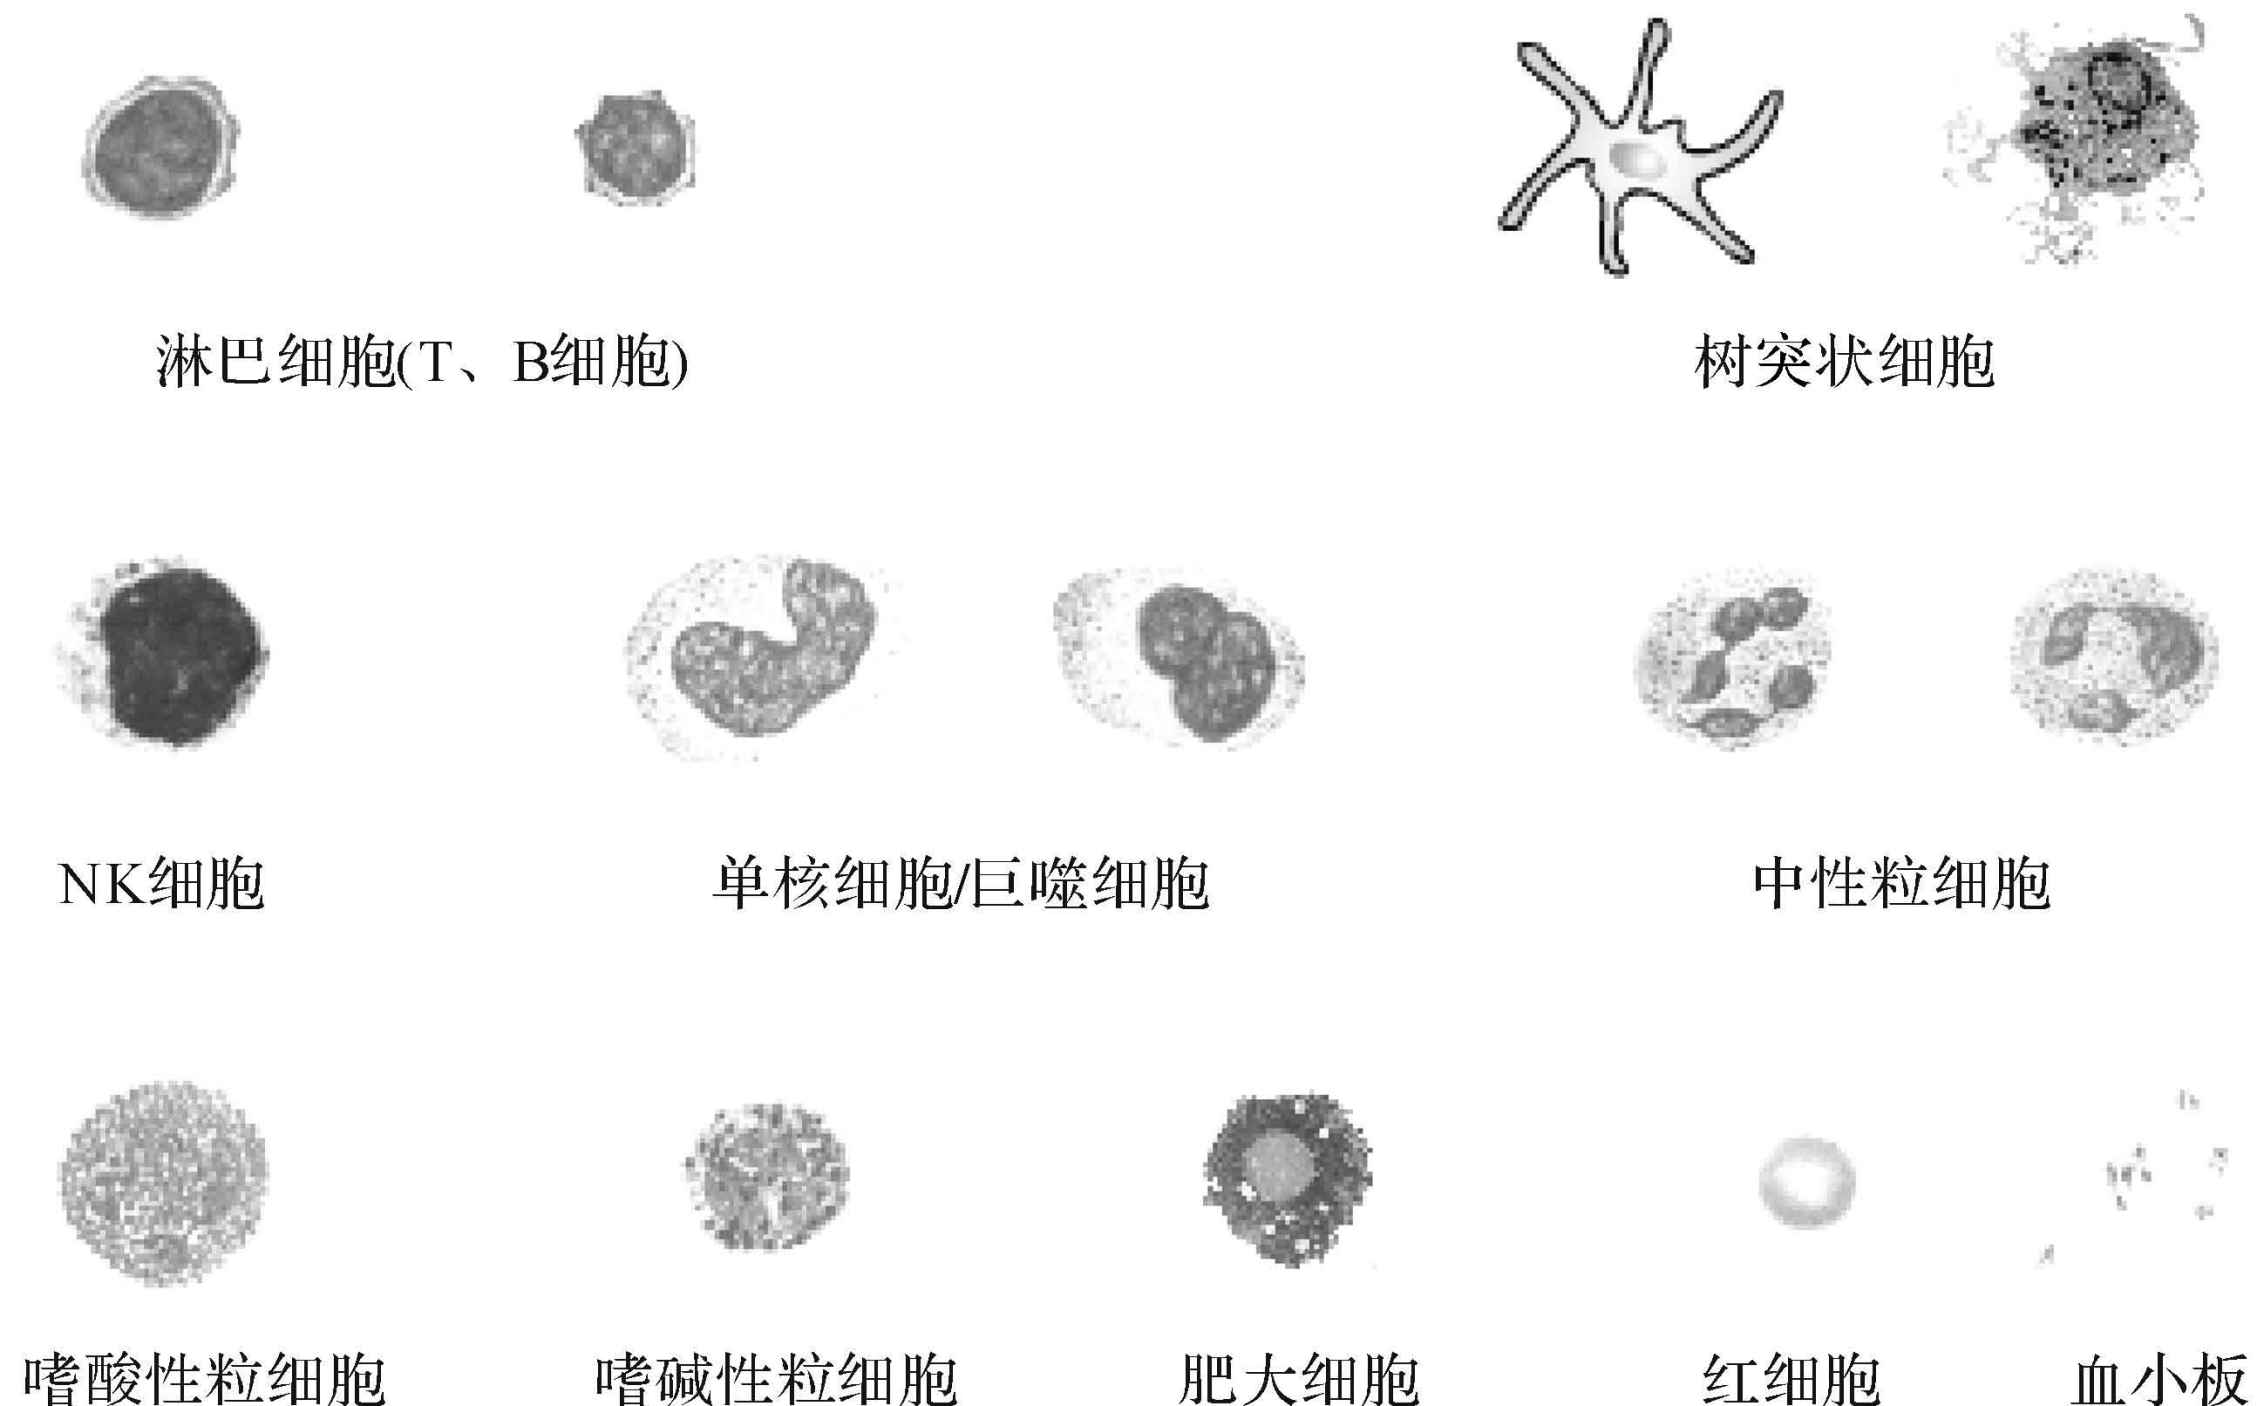
\includegraphics[width=.6\textwidth]{./images/Image00038.jpg}
 \caption{各种免疫细胞}
 \label{fig2-13}
  \end{figure} 


\subsection{造血干细胞}

造血干细胞(hemopoietic stem
cell,HSC)又称多能干细胞,是存在于造血组织中的一群原始造血细胞。也可以说,它是一切血细胞(其中大多数是免疫细胞)的原始细胞。由造血干细胞定向分化、增殖为不同的血细胞系,并进一步生成血细胞。人类造血干细胞首先出现于胚龄第2~3周的卵黄囊,在胚胎早期(第2~3月)迁至肝、脾,第5个月又从肝、脾迁至骨髓。在胚胎末期一直到出生后,骨髓成为造血干细胞的主要来源,具有多潜能性,即具有自身复制和分化两种功能。


\subsection{淋巴细胞}

淋巴细胞(lymphocyte)是构成免疫系统的主要细胞类别,占外周血白细胞总数的20%~45%,成年人体内约有10\textsuperscript{12}
个淋巴细胞。淋巴细胞可分为许多表型与功能均不同的群体,如T细胞、B细胞、NK细胞等;T细胞和B细胞还可进一步分为若干亚群。这些淋巴细胞及其亚群在免疫应答过程中相互协作、相互制约,共同完成对抗原物质的识别、应答和清除,从而维持机体内环境的稳定。

其特点是:未活化淋巴细胞在抗原的刺激下转变为淋巴母细胞,再进一步转变为效应T细胞与记忆细胞。可分群为:
\begin{itemize}
\item T细胞:细胞膜上表达CD3分子和TCR
\item B细胞:细胞膜上表达BCR
\item NK细胞:细胞膜上表达CD56和CD16
\end{itemize}

(一)T淋巴细胞

T淋巴细胞(T
lymphocyte)简称T细胞,其介导细胞免疫应答,并在机体针对TD抗原的体液免疫应答中发挥重要的辅助作用。骨髓中的淋巴样前体细胞(lymphoid
precursor)进入胸腺,经历一系列有序的分化过程,才能发育为成熟T细胞。T细胞乃高度异质性的细胞群,依据其表面标志及功能特征,可分为若干亚群。在免疫应答过程中,各亚群T细胞相互协作,共同发挥重要的免疫学功能。

1.T细胞的表面标志

T细胞表面标志即其膜分子(如图\ref{fig2-14}所示),是T细胞识别抗原、与其他免疫细胞相互作用、接受信号刺激并产生应答的物质基础,亦是鉴别和分离T细胞的重要依据。在诸多表面标志中,TCR、CD3分子是外周血成熟T细胞各亚群的共有标志。

(1)T细胞表面受体(surface antigen):T细胞抗原受体(T cell antigen
receptor,TCR)、细胞因子受体(cytokine receptor,CKR)、丝裂原受体。

(2)T细胞表面抗原(surface antigen):MHC抗原、分化抗原(CD分子)等。

\begin{figure}[!htbp]
 \centering
 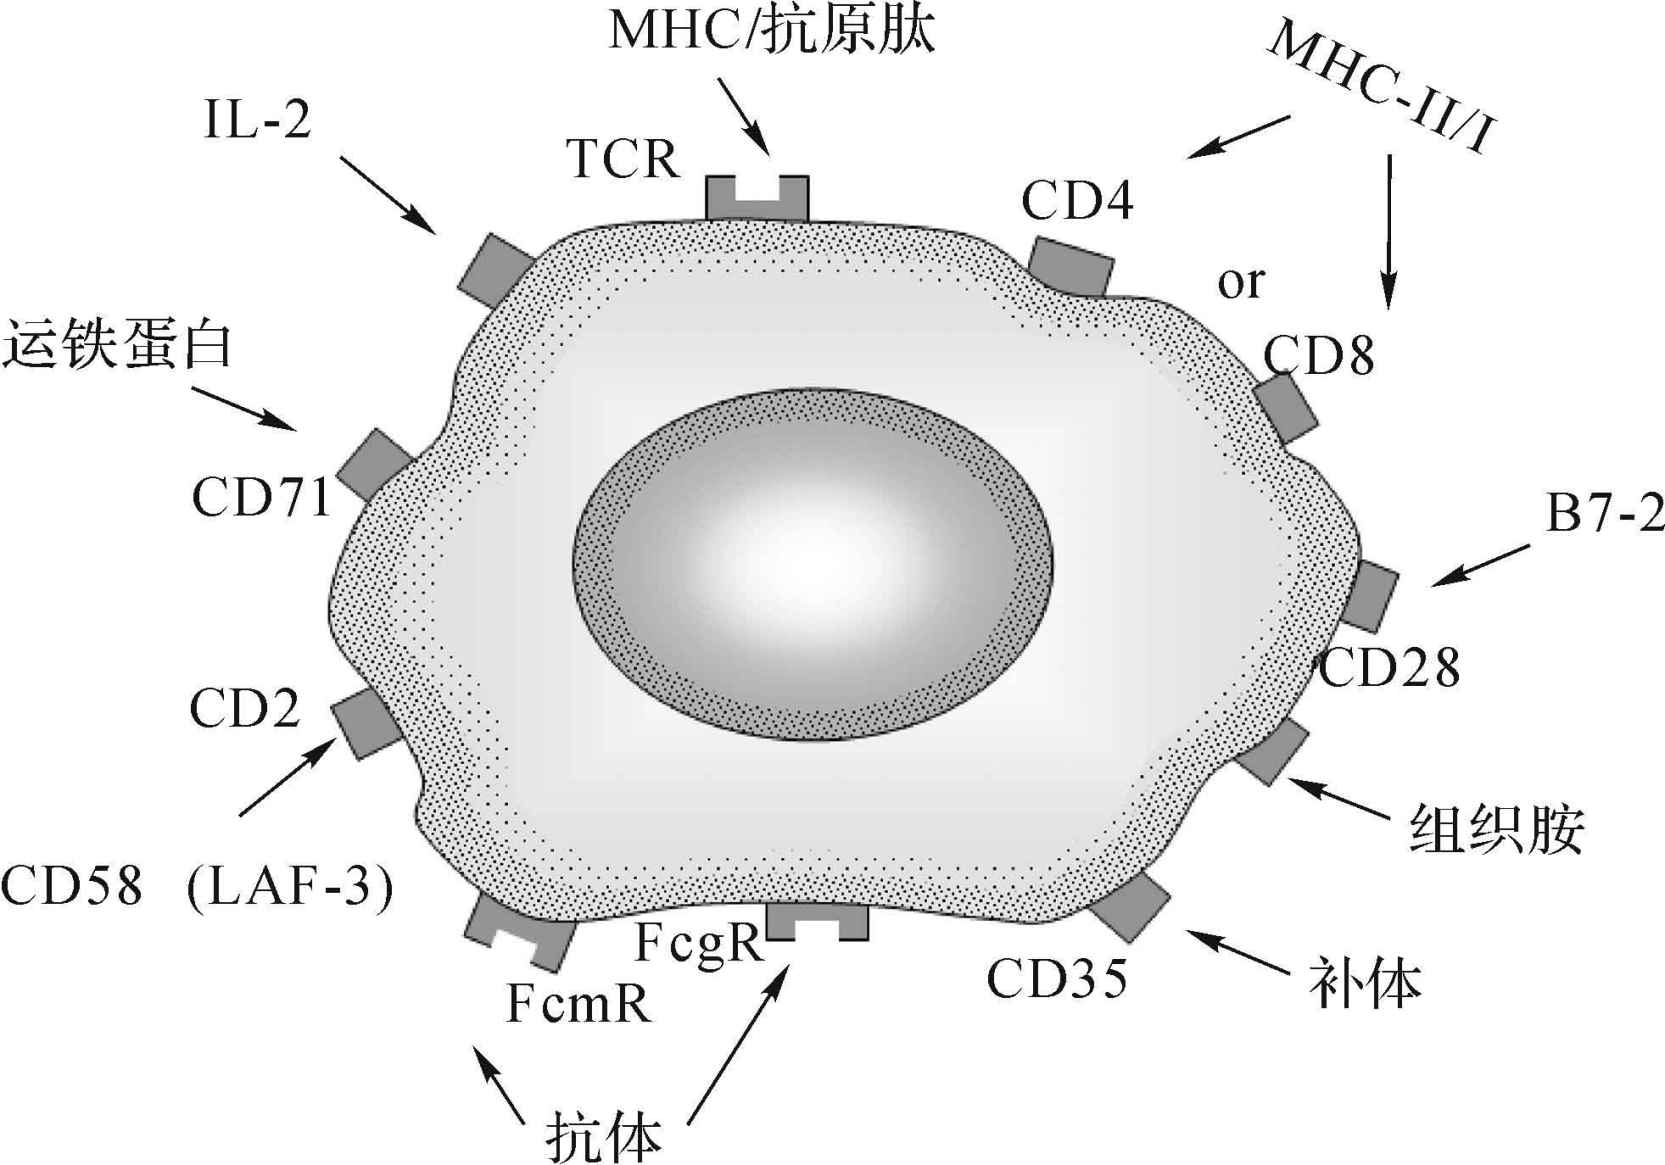
\includegraphics{./images/Image00039.jpg}
 \caption{T细胞表面标志}
 \label{fig2-14}
  \end{figure} 

2.T细胞亚群及其功能

人类的T细胞不是均一的群体,根据表面标志和功能可为五个亚群:

CD4\textsuperscript{+}
T(初始T细胞,Th1细胞,Th2细胞):占T细胞的65\%左右,它的重要标志是表面有CD4抗原。Th细胞能识别抗原,分泌多种淋巴因子,它既能辅助B细胞产生体液免疫应答,又能辅助T细胞产生细胞免疫应答,是扩大免疫应答的主要成分,它还具有某些细胞免疫功能。

CD8\textsuperscript{+}
T(杀伤性T细胞,抑制性T细胞):杀伤性T细胞占T细胞的20%~30%,表面也有CD8抗原。杀伤性T细胞能识别结合在MHC-Ⅰ类抗原上的异抗原,在异抗原的刺激下可增殖形成大量效应性杀伤性T细胞,能特异性地杀伤靶细胞,是细胞免疫应答的主要成分。抑制性T细胞占T细胞的10%左右,表面有CD8抗原。抑制性T细胞常在免疫应答的后期增多,它分泌的抑制因子可减弱或抑制免疫应答。

(1)初始T细胞(naive T
cell):指未完全分化的Th细胞,是Th1、Th2细胞的前体,分泌低水平的IL-4和IFN-γ。

功能:调节体液免疫应答和细胞免疫应答,分化产生Th1、Th2细胞,T细胞的分化如图\ref{fig2-15}所示。

\begin{figure}[!htbp]
 \centering
 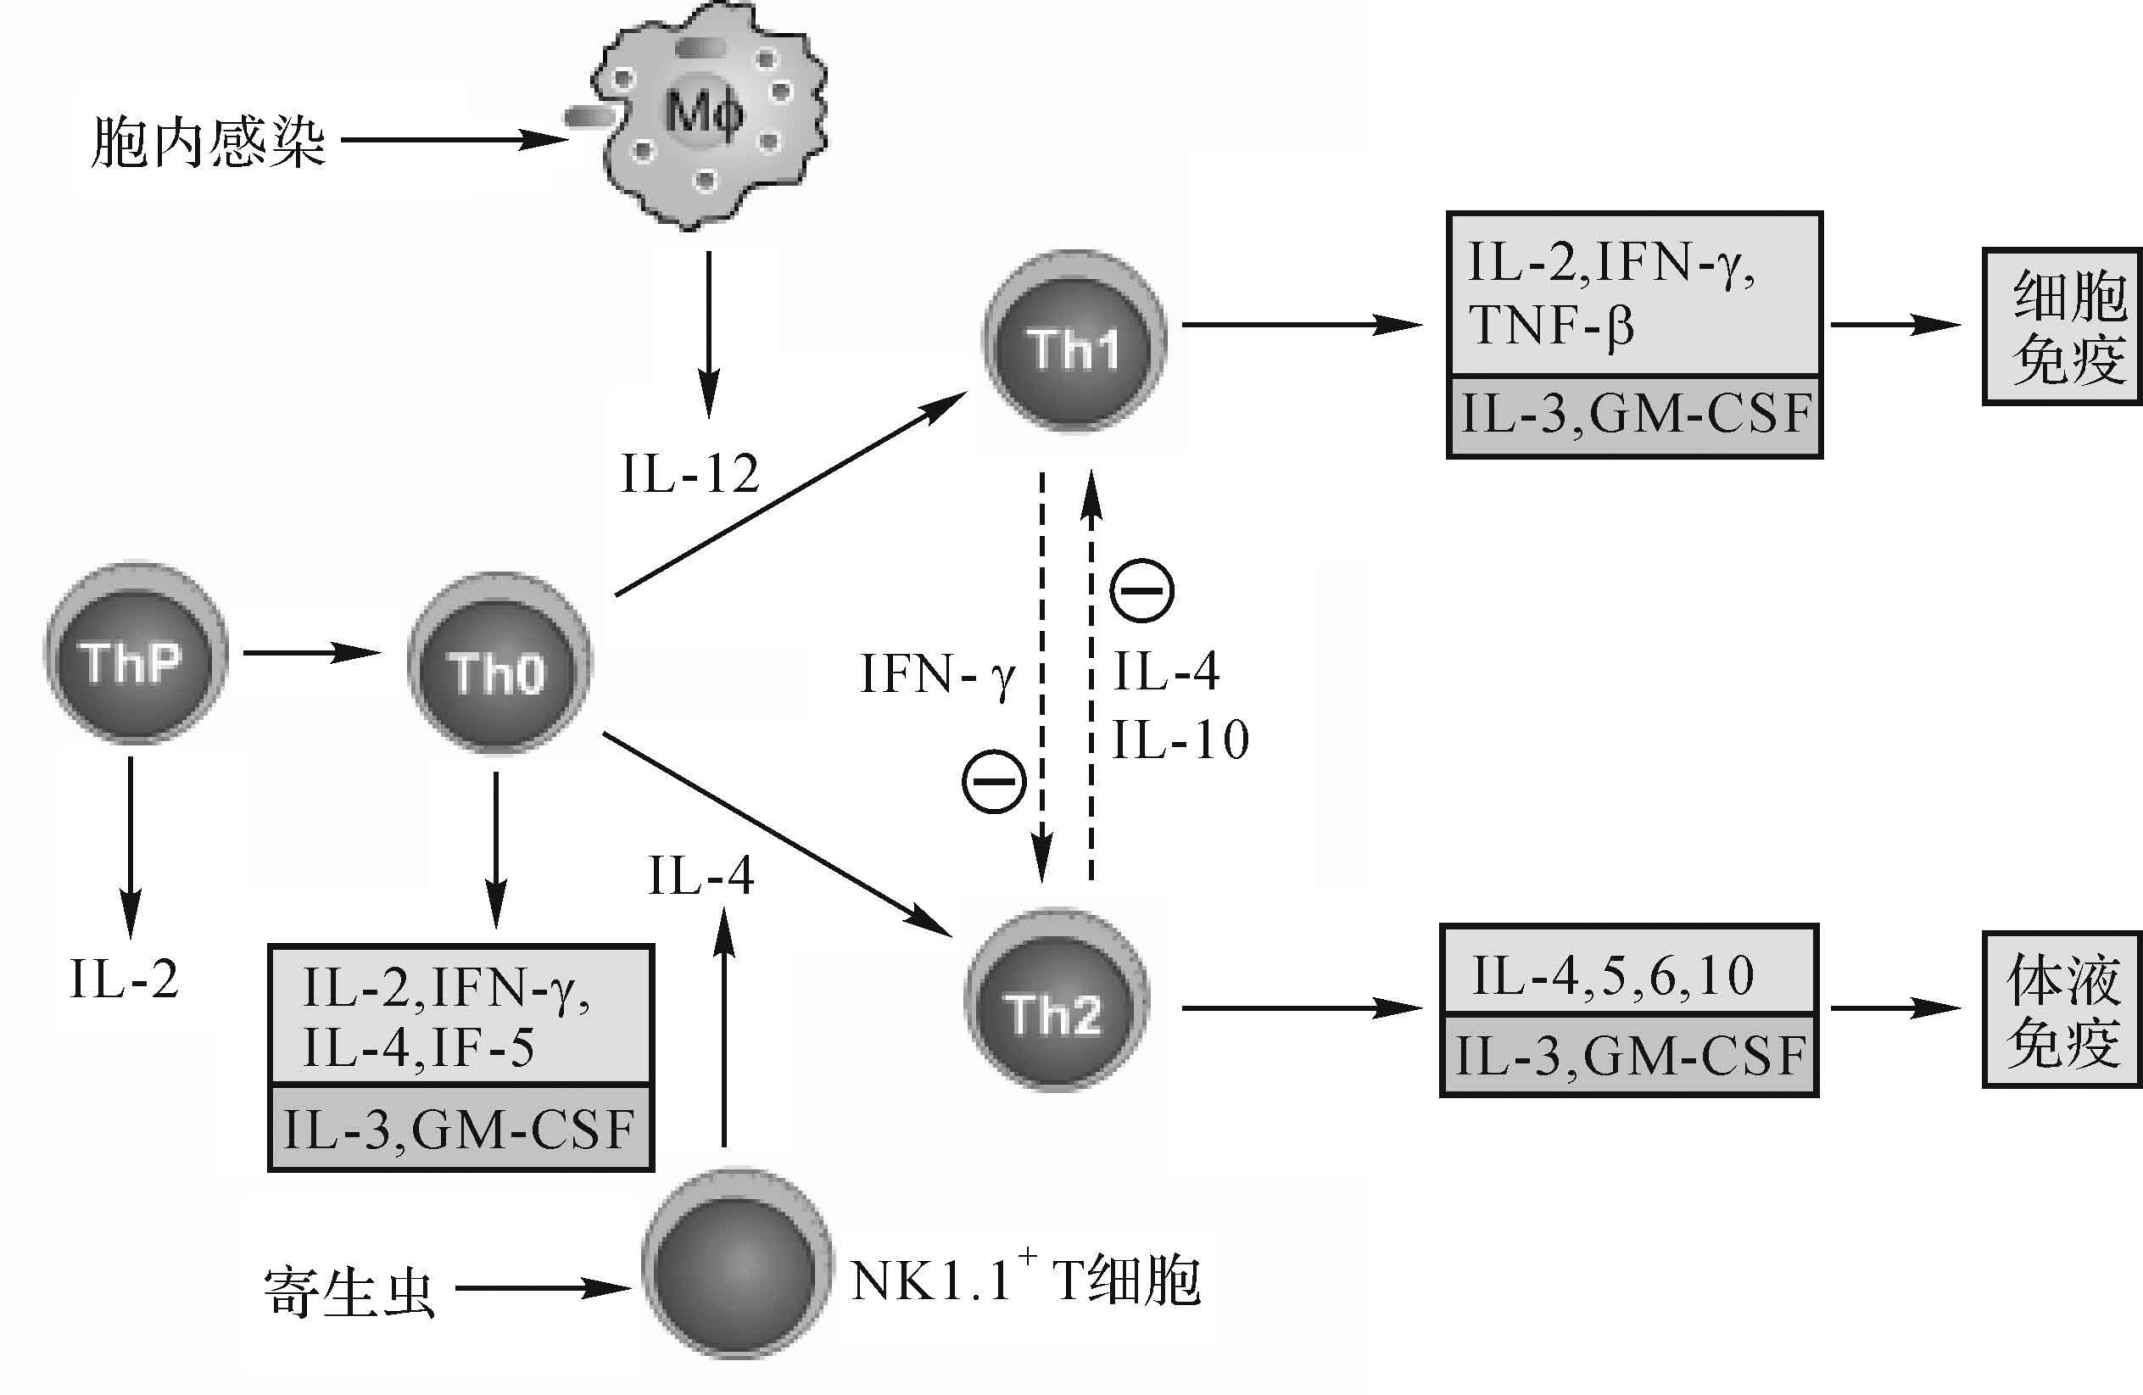
\includegraphics{./images/Image00040.jpg}
 \caption{T细胞的分化}
 \label{fig2-15}
  \end{figure} 

按分泌的细胞因子不同可将Th细胞分为两个不同的亚群:分泌IFN-γ、IL-2的称为TH1细胞,分泌IL-4、IL-5的称为Th2细胞。

(2)Th1细胞:初始T细胞在IL-12作用下转变为Th1细胞。

Th1细胞功能:释放IL-2、IFN-γ和TNF,引起炎症反应或迟发型超敏反应,称为炎症性T细胞。参与细胞免疫应答及迟发型超敏反应。在抗胞内病原微生物等感染中起重要作用。Th1细胞持续性强应答,可能与器官特异性自身免疫病、接触性皮炎、不明原因的慢性炎症性疾病、迟发型超敏反应性疾病、急性同种异体移植排斥反应等的发生有关。

(3)Th2细胞:初始T细胞在IL-4作用下转变为Th2细胞。

释放IL-4、5、6、10,诱导B细胞增殖分化、合成并分泌抗体,引起体液免疫应答或速发型超敏反应(图\ref{fig2-16})。

\begin{figure}[!htbp]
 \centering
 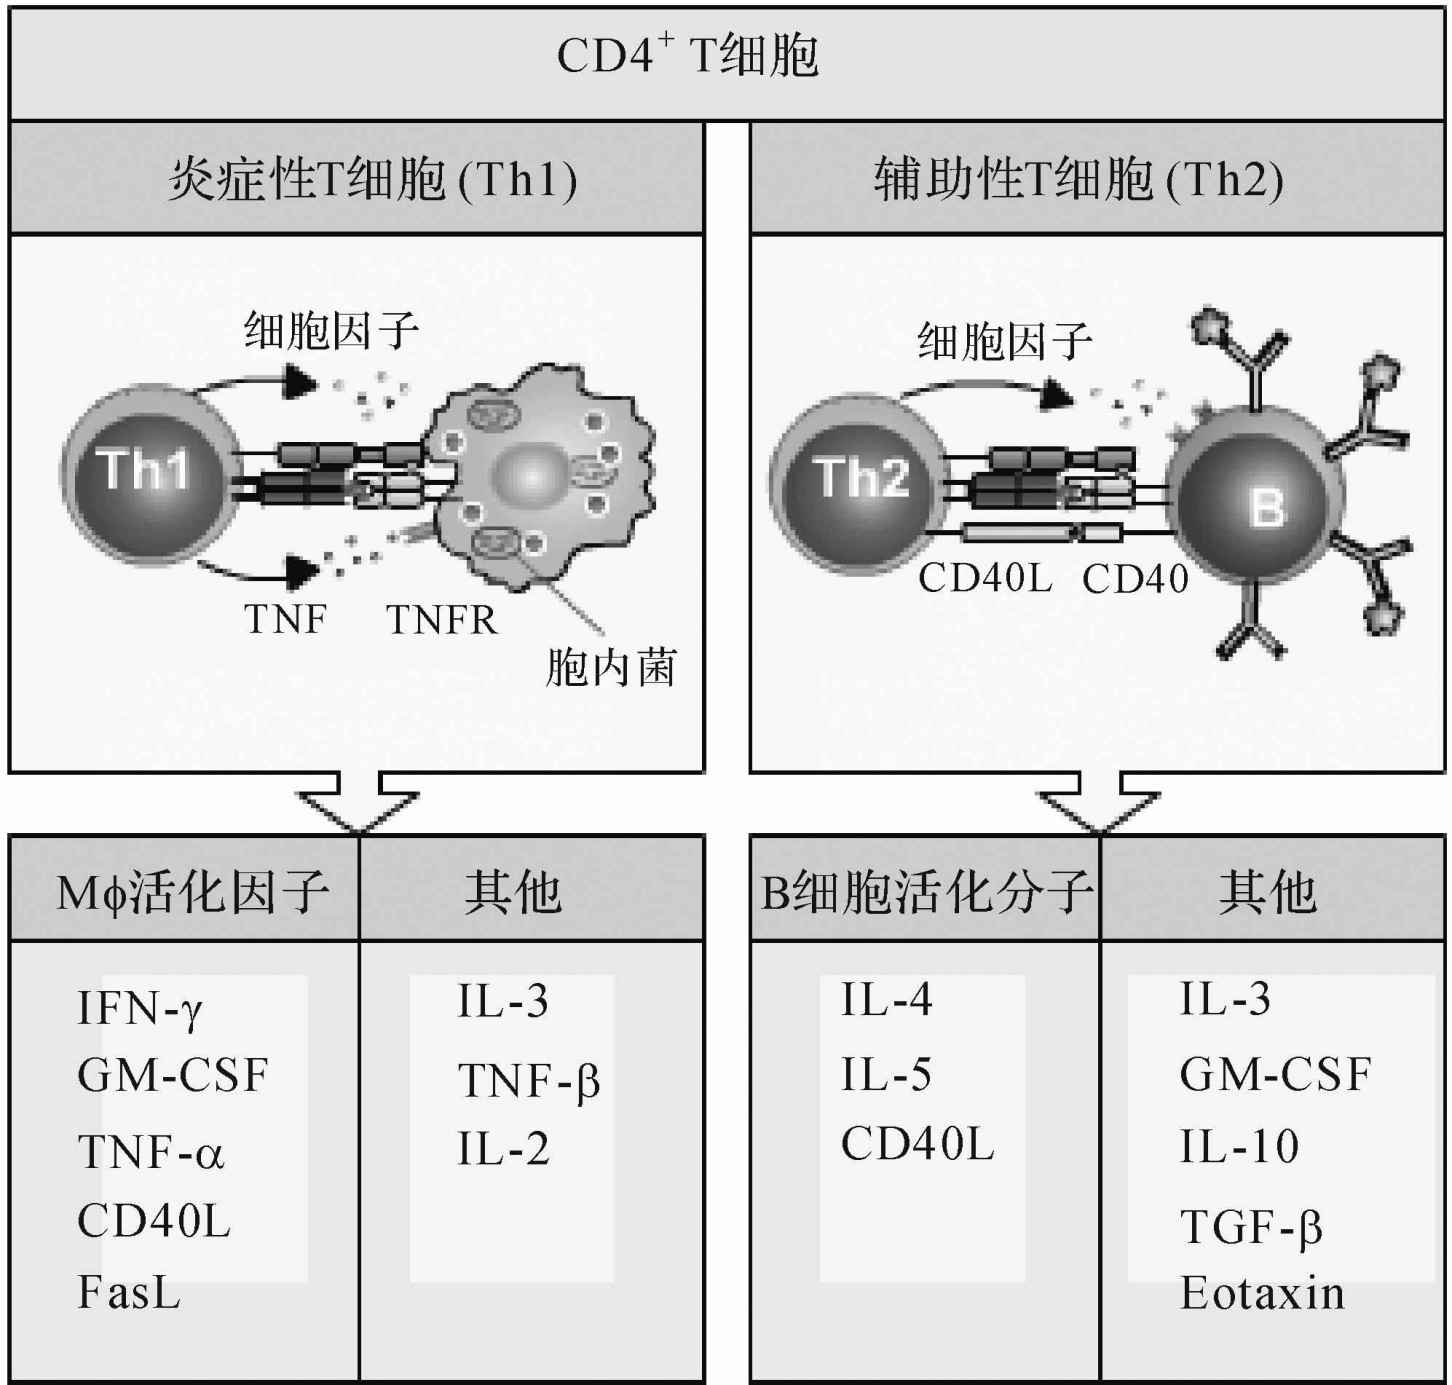
\includegraphics[width=.5\textwidth]{./images/Image00041.jpg}
 \caption{Th1、Th2淋巴细胞的功能}
 \label{fig2-16}
  \end{figure} 

(4)杀伤性T细胞(CTL):也叫细胞毒性T细胞,是效应T细胞,经抗原致敏后,CTL
的TCR特异性识别靶细胞(如病毒感染细胞、肿瘤细胞、同种异体移植物细胞等)表面的抗原肽/MHC-I类分子复合物。活化CTL
杀伤效应的主要机制为:①分泌穿孔素(perforin)、颗粒酶(granzyme)或淋巴毒素等直接杀伤靶细胞;②通过高表达FasL导致Fas阳性的靶细胞凋亡。CTL参与的免疫效应为抗病毒感染、抗肿瘤和介导同种异体移植排斥反应等(图\ref{fig2-17})。

\begin{figure}[!htbp]
 \centering
 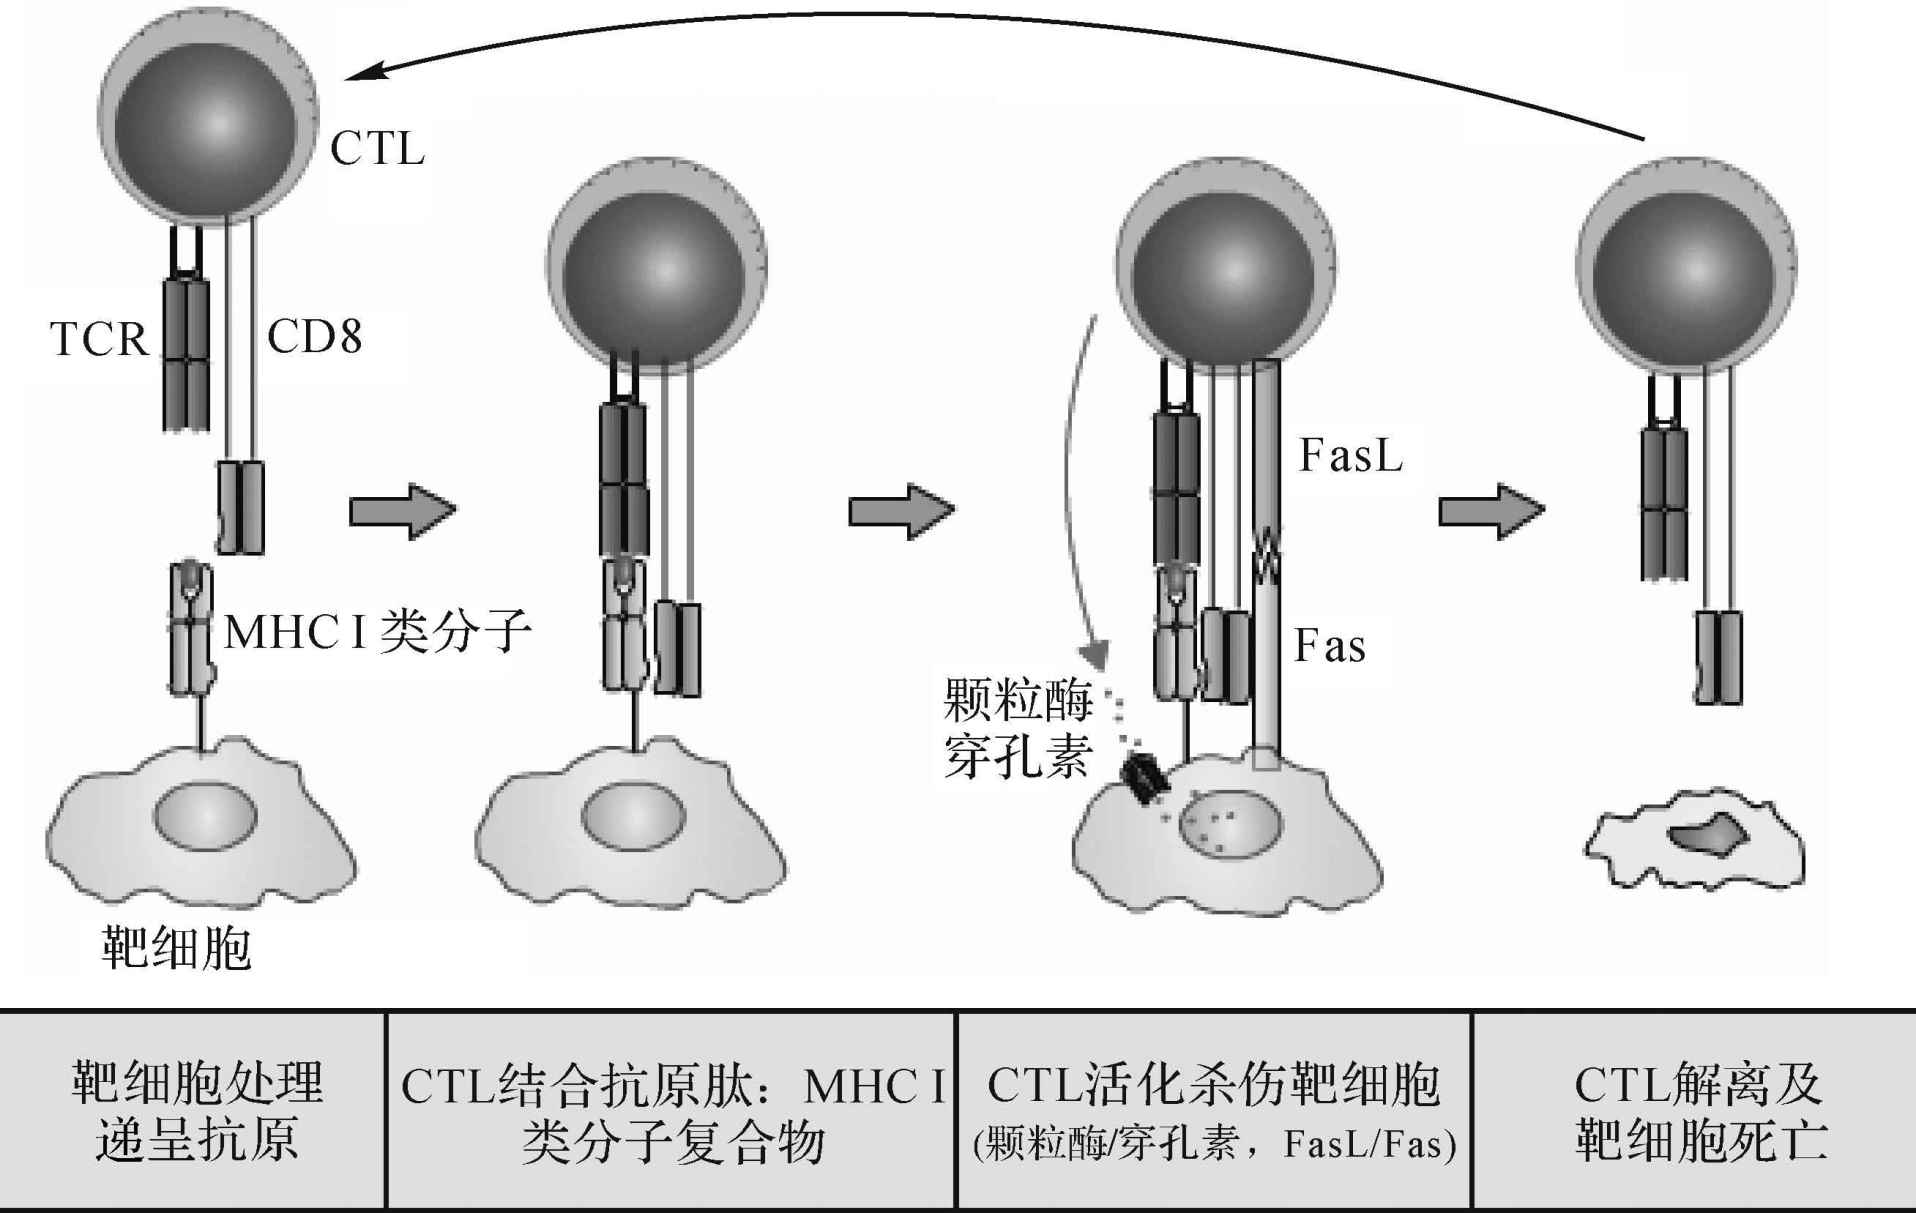
\includegraphics[width=.5\textwidth]{./images/Image00042.jpg}
 \caption{CTL的免疫效应}
 \label{fig2-17}
  \end{figure} 

(5)Ts细胞(suppressor T cell,Ts):具有抑制体液免疫和细胞免疫的功能。

(二)B淋巴细胞

B淋巴细胞(B
lymphocyte)是始祖B淋巴细胞在骨髓(人、动物)、法氏囊(禽)中发育、分化、成熟,产生抗体,也称骨髓或囊依赖性细胞,是体内唯一能产生抗体(Ig)的细胞,主要执行体液免疫,也具有抗原递呈功能。外周血中占淋巴细胞总数10\%~15\%,简称B细胞,是由哺乳动物骨髓或鸟类法氏囊中的淋巴样前体细胞分化成熟而来。

1.B细胞的表面标志

B细胞表面标志如图\ref{fig2-18}所示。

\begin{figure}[!htbp]
 \centering
 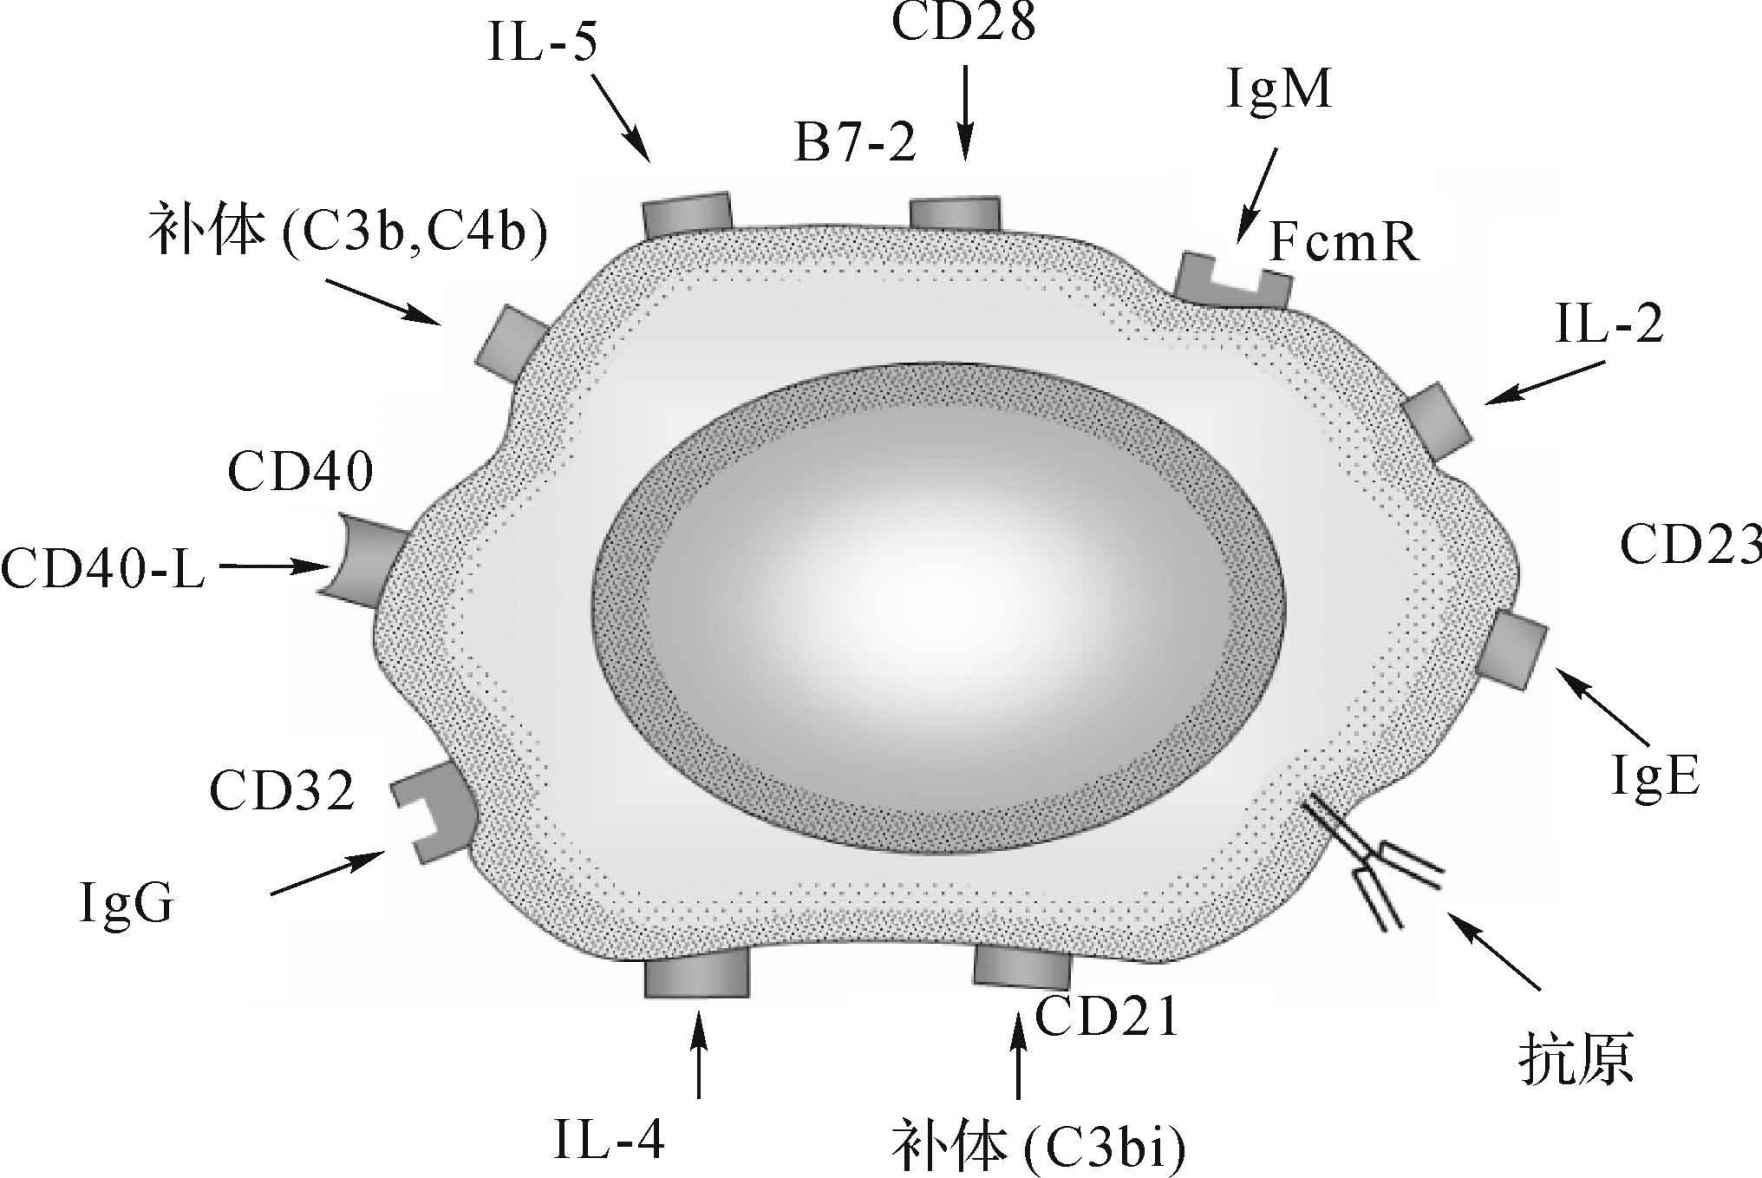
\includegraphics[width=.5\textwidth]{./images/Image00043.jpg}
 \caption{B细胞表面标志}
 \label{fig2-18}
  \end{figure} 

(1)B细胞抗原受体(B-cell antigen
receptor,BCR):BCR是嵌入细胞膜类脂分子中的膜表面免疫球蛋白(mIg),乃B细胞的特征性表面标志,也是B细胞特异性识别不同抗原表位的分子基础。

(2)细胞因子受体:B细胞表面表达IL-1R、IL-2R、IL-4R、IL-5R、IL-6R、IL-7R及IFN-γR等多种细胞因子受体。细胞因子通过与B细胞表面相应受体结合而参与或调节B细胞活化、增殖和分化。

(3)补体受体(CR):多数B细胞表面表达CR1和CR2(即CD35和CD21)。CR1主要见于成熟B细胞,其在B细胞活化后表达增高。CR1与相应配体结合可促进B细胞活化。CR2(CD21)是EB病毒受体,在体外应用EB病毒感染B细胞可使之转化为B淋巴母细胞系,从而达到永生化(immortalized)。

(4)Fc受体:多数B细胞表达IgG Fc受体Ⅱ(FcγRⅡ),可与免疫复合物中的IgG
Fc段结合,有利于B细胞捕获和结合抗原,并促进B细胞活化和抗体产生。

(5)丝裂原受体:某些丝裂原通过与B细胞表面相应受体结合,使其被激活并增殖分化为淋巴母细胞,可用于检测B细胞功能状态。美洲商陆(PWM)对T细胞和B细胞均有致有丝分裂作用;脂多糖(LPS)是常用的小鼠B细胞丝裂原。

2.细胞表面抗原

(1)MHC抗原:B细胞可表达MHC-Ⅰ类和MHC-Ⅱ类抗原。MHC-Ⅱ类抗原可与Th细胞表面CD4结合,增强B细胞与Th细胞间的黏附作用,并参与抗原递呈和淋巴细胞激活。

(2)CD抗原:B细胞分化发育的不同阶段,其CD抗原的表达各异,有CD19、CD20、CD21、CD40/CD40L、CD80(B7-1)/CD86(B7-2)。

3.B细胞亚群及功能

根据是否表达CD5分子,可将人B细胞分为B1(CD\textsuperscript{+}
\textsubscript{5} )和B2(CD\textsuperscript{-} \textsubscript{5}
)细胞。

(1)B1细胞亚群:B1细胞在个体发育过程中出现较早,是由胚胎期或出生后早期的前体细胞分化而来,其发生不依赖于骨髓细胞。B1细胞产生后,成为具有自我更新(self-renewal)能力的长寿细胞,主要分布于胸腔、腹腔和肠壁固有层中。B1细胞的抗原识别谱较窄,主要针对属于TI-2抗原的多糖类物质,尤其是某些菌体表面共有的多糖抗原(如肺炎球菌荚膜多糖等)。B1细胞的功能特点是:主要产生IgM类的低亲和力抗体;不发生抗体类别转换;无免疫记忆。

(2)B2细胞亚群:B2细胞即通常所称的B细胞,是参与体液免疫应答的主要细胞类别。它是由骨髓中多能造血干细胞分化而来,属形态较小、比较成熟的B细胞,在体内出现较晚,定位于外周淋巴器官。B2细胞的主要生物学功能为:参与体液免疫应答、抗原递呈、免疫调节。

(三)自然杀伤细胞

自然杀伤细胞(natural
killer,NK)是一类独立的淋巴细胞群,其不同于T细胞和B细胞,不表达特异性抗原识别受体(图\ref{fig2-19})。NK细胞胞浆内有许多嗜苯胺颗粒,故又称为大颗粒淋巴细胞(large
granular
lymphocyte)。NK细胞无须抗原预先致敏即可直接杀伤某些靶细胞,包括肿瘤细胞、病毒或细菌感染的细胞以及机体某些正常细胞(图\ref{fig2-20})。
\begin{figure}[!htbp]
    \centering
    \begin{minipage}[b]{0.45\textwidth} 
      \centering
        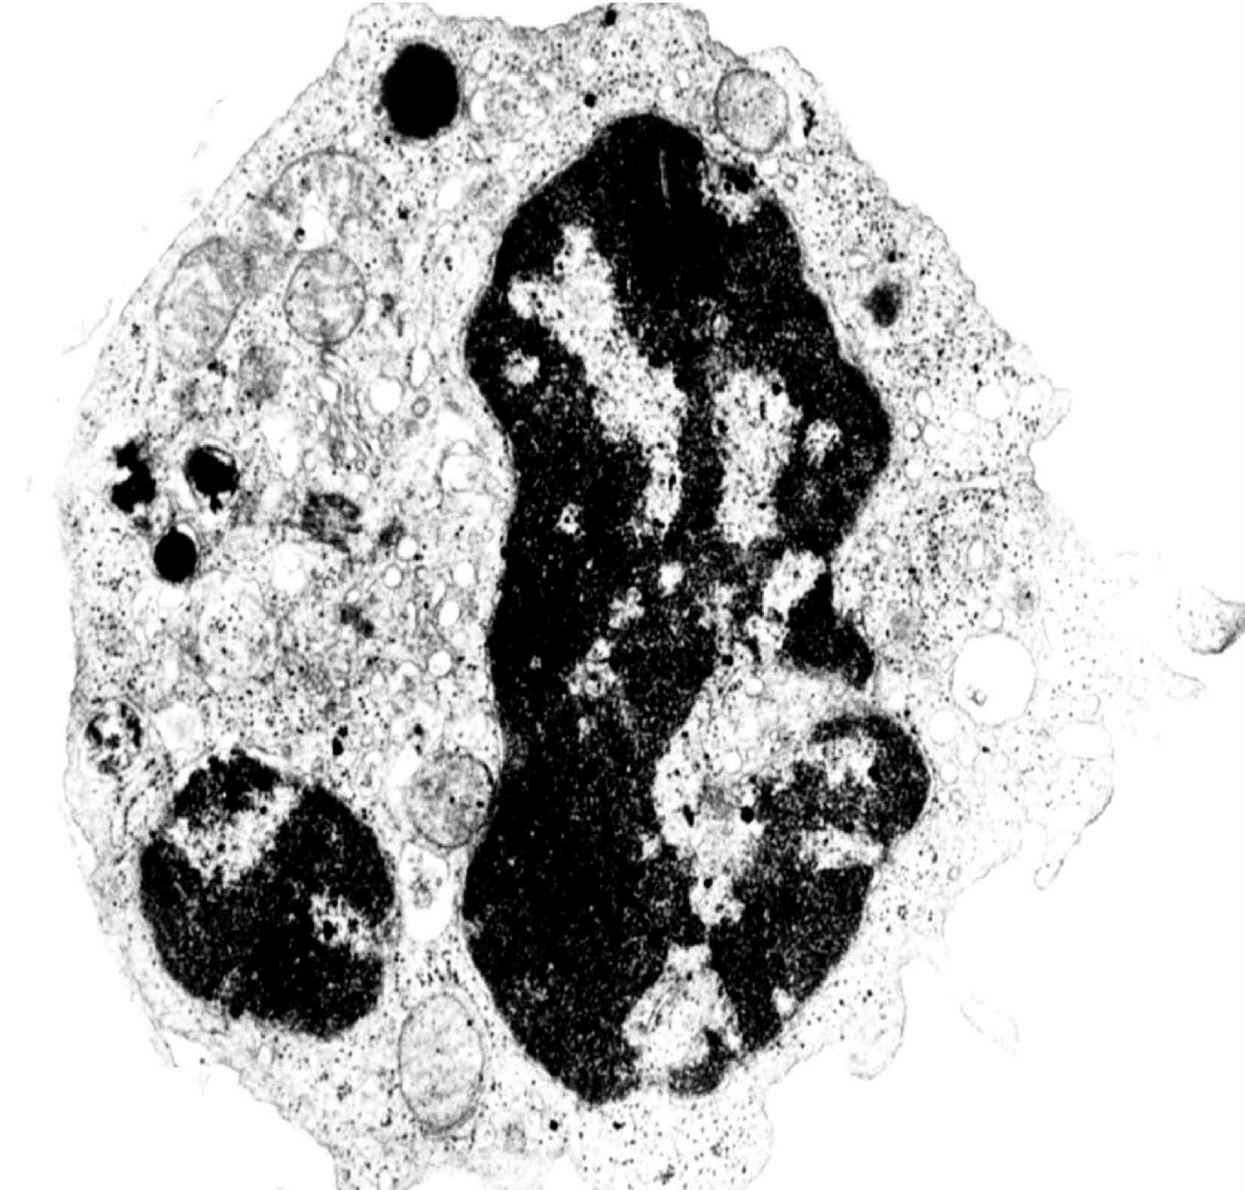
\includegraphics[height=0.12\textheight]{./images/Image00044.jpg}
        \captionsetup{justification=centering}
        \caption{自然杀伤细胞}
        \label{fig2-19}
    \end{minipage}
%	\end{figure} 
	%\FloatBarrier
%\begin{figure}[!htbp]
%    \centering
%\hspace{0.04\textwidth}%
\begin{minipage}[b]{0.45\textwidth} 
  \centering
    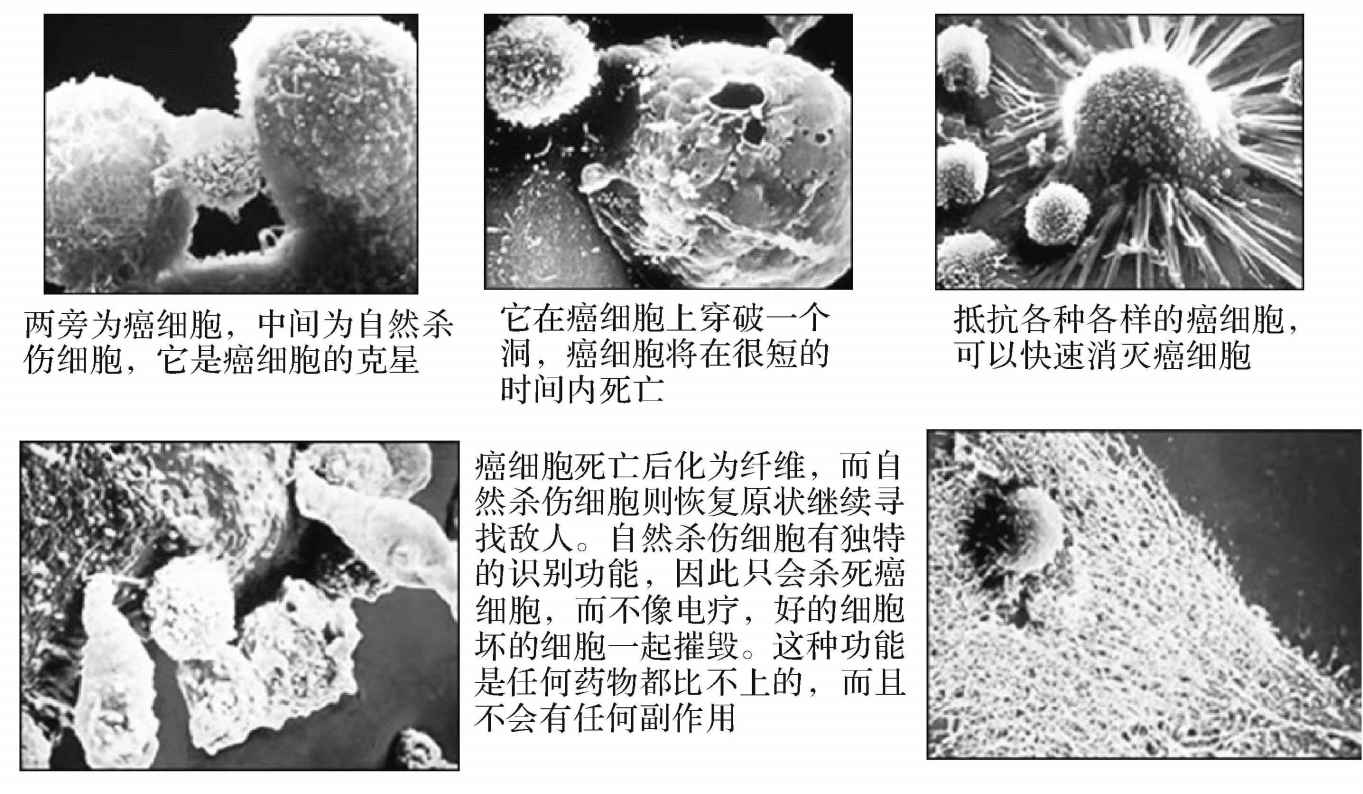
\includegraphics[height=0.2\textheight]{./images/Image00045.jpg}
    \captionsetup{justification=centering}
    \caption{NK细胞杀死癌细胞}
    \label{fig2-20}
\end{minipage}
\end{figure} 

1.来源及分布

NK细胞是由骨髓中的共同淋巴样祖细胞(commen lymphoid
progenitor,CLP)分化而来,其发育、成熟可能循骨髓途径或胸腺途径。人类和小鼠NK细胞主要分布于脾脏(占脾细胞总数3\%~4\%)和外周血(占淋巴细胞总数5%~7%),在淋巴结以及其他组织内(如肺脏等)也有少量NK细胞存在。近年发现,肝脏中NK细胞占淋巴细胞总数50\%以上,其生物学意义有待阐明。

2.功能

(1)能非特异性杀伤某些肿瘤细胞和病毒感染的靶细胞,具有抗肿瘤、抗感染的功能。

(2)NK细胞可产生IL-1、IFN-r、TNF等,有免疫调节作用。

(3)参与移植排斥反应、自身免疫病、超敏反应的发生。


\subsection{单核吞噬细胞系统}

单核吞噬细胞系统(mononuclear phagovyte
system,MPS)包括单核细胞、巨噬细胞,是体内具有最活跃生物学功能的细胞类型之一(图\ref{fig2-21})。

\begin{figure}[!htbp]
 \centering
 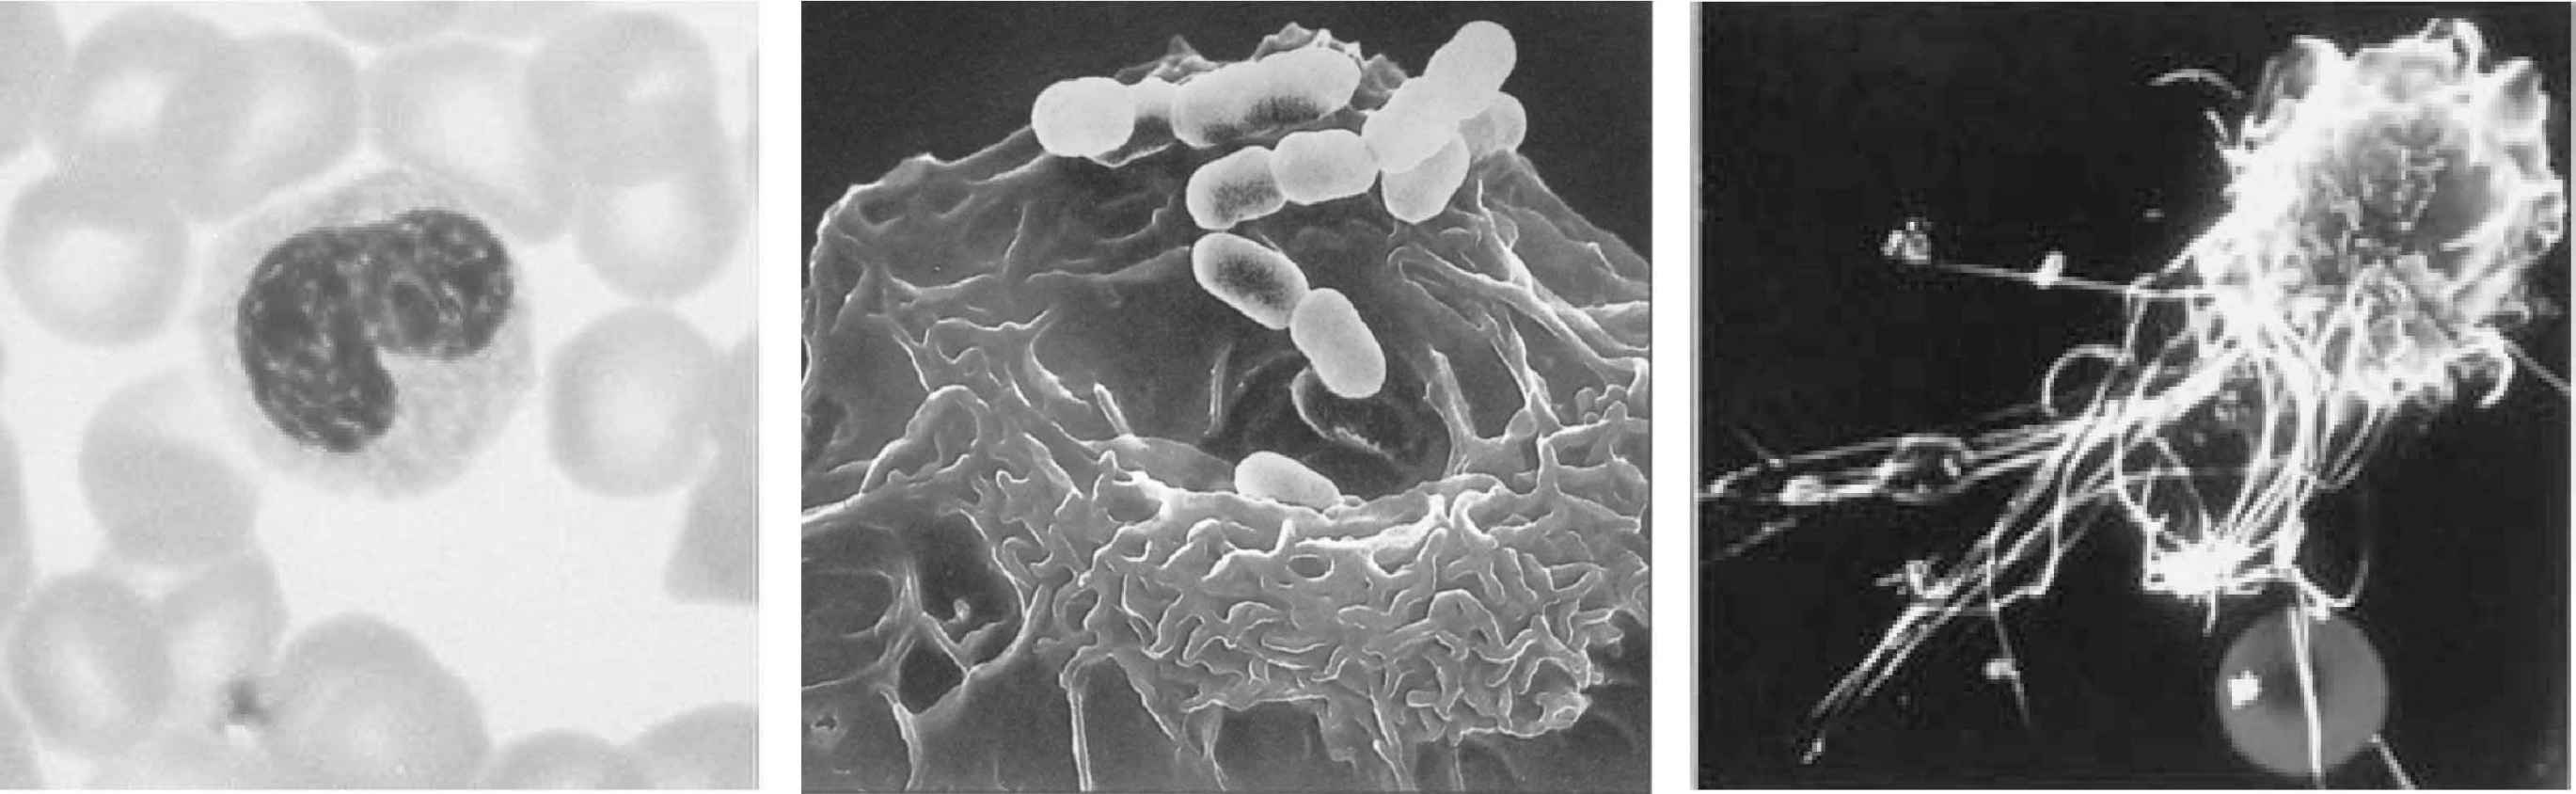
\includegraphics[width=.7\textwidth]{./images/Image00046.jpg}
 \caption{单核吞噬细胞}
 \label{fig2-21}
  \end{figure} 

1.表面标志:表达多种表面标志,并借此发挥各种生物学功能,如MHC分子、黏附分子等。这些表面标志不仅参与细胞黏附及对颗粒抗原的摄取、递呈,也介导相应配体触发的跨膜信号转导,并影响细胞分化和发育等。

2.产生多种酶及分泌产物:单核吞噬细胞能产生各种溶酶体酶、溶菌酶、髓过氧化物酶等,还能产生和分泌近百种生物活性物质,如细胞因子(IL-1、IL-6、IL-12等)、补体成分(C1、P因子等)、凝血因子,以及前列腺素、白三烯、血小板活化因子、ACTH、内啡肽等活性产物。

3.功能:具有抗感染、抗肿瘤、免疫调节的作用。


\subsection{其他免疫细胞}

(一)中性粒细胞

中性粒细胞表面具有IgFc受体和C3b受体,具有高度趋化性和非特异性功能,有抗感染作用(图\ref{fig2-22})。

\begin{figure}[!htbp]
 \centering
 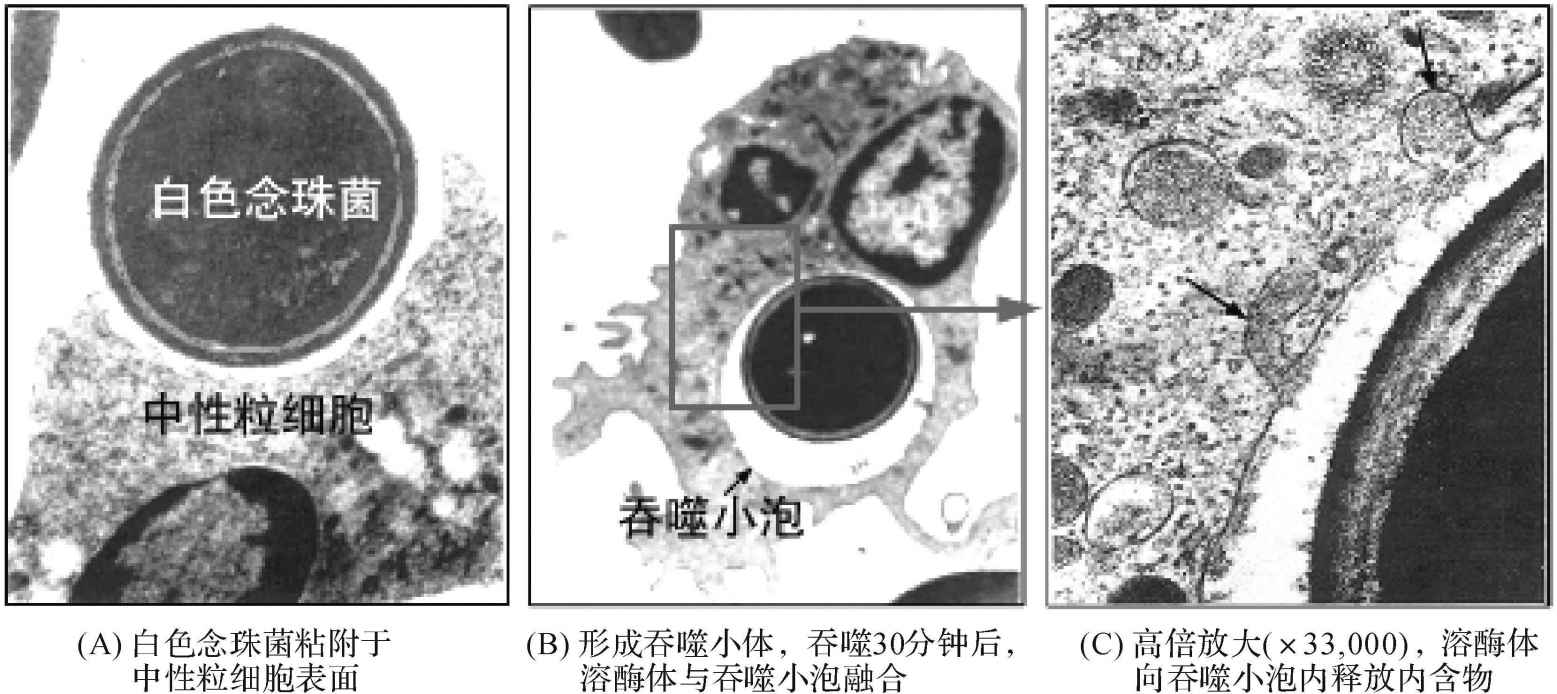
\includegraphics[width=.7\textwidth]{./images/Image00047.jpg}
 \caption{中性粒细胞的吞噬作用}
 \label{fig2-22}
  \end{figure} 

(二)嗜酸性粒细胞

嗜酸性粒细胞具有IgFc受体,参与IgE介导的ADCC效应;具有吞噬作用,抗寄生虫和对I型超敏反应的负调节作用。

(三)嗜碱性粒细胞与肥大细胞

嗜碱性粒细胞与肥大细胞表面具有IgE的Fc受体,能参与I型超敏反应、抗肿瘤作用(图\ref{fig2-23})。

\begin{figure}[!htbp]
 \centering
 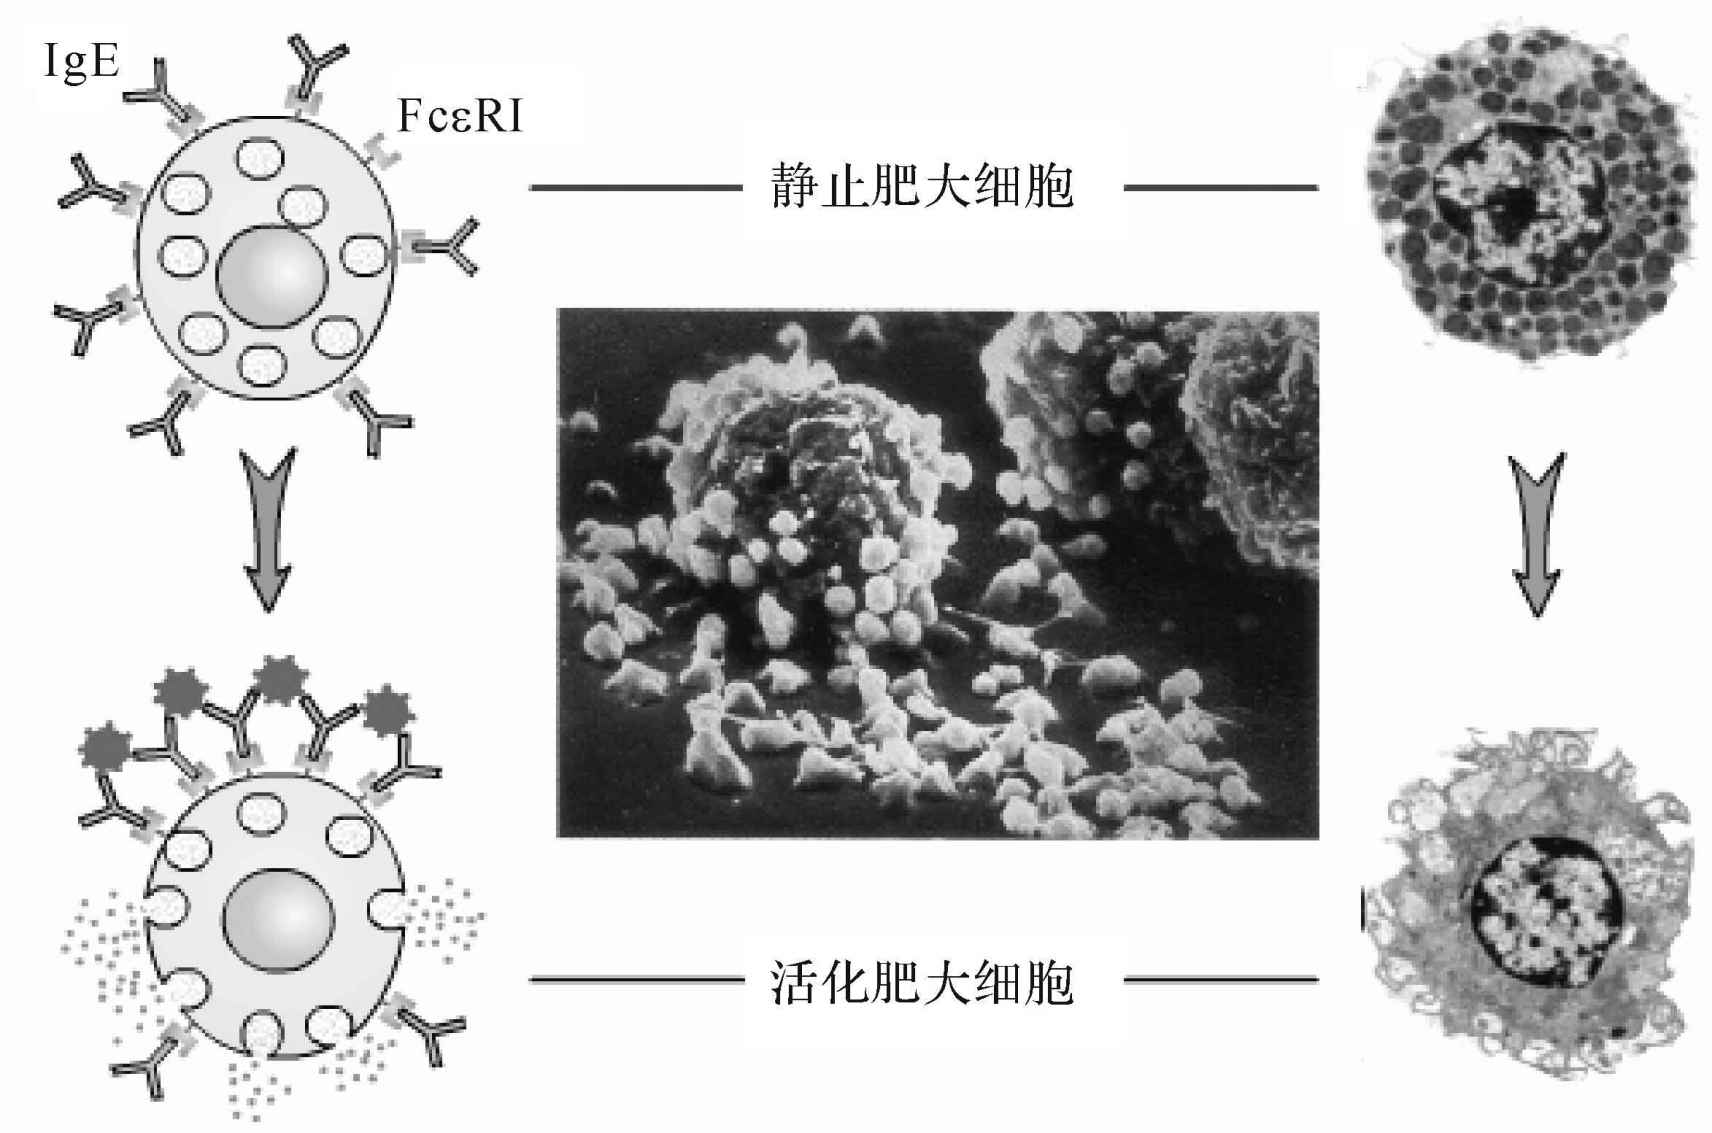
\includegraphics[width=.6\textwidth]{./images/Image00048.jpg}
 \caption{肥大细胞参与Ⅰ型超敏反应}
 \label{fig2-23}
  \end{figure} 

(四)红细胞

1.红细胞免疫的物质基础

① 红细胞CR1分子------结合C3b/C4b;

② 红细胞CD58分子------即LFA-3,与CD2互为配体和受体;

③ 红细胞CD59分子------阻止C9与C5B678结合,促进T细胞有丝分裂;

④ 红细胞CD55分子------即衰变加速因子DAF;

⑤ 红细胞CD44分子------参与T、B的分化、成熟、活化,细胞黏附;

⑥ 红细胞NK细胞增强因子------增强NK细胞的毒性;

⑦ 红细胞趋化因子受体------参与调控炎症反应。

2.红细胞在整体免疫反应中的作用

① 增强吞噬作用;

② 清除循环免疫复合物;

③ 识别和携带抗原;

④ 免疫调节作用;

⑤ 效应细胞的作用。

\section{思考练习与课外阅读}
\noindent\textbf{【理解与思考】}

1.你能向一位没有免疫学知识的人,形象地解说机体免疫系统的构成及其作用吗?

2.你能描绘出体内淋巴细胞的一生历程吗?

3.如果你是一病原微生物,进入机体后你能遭遇哪些危险?

4.如果你是一免疫细胞,你又是如何保证机体健康的?

5.以红细胞的口气,向别人叙述一下你在人体内的贡献。

\noindent\textbf{【课外拓展】}

1.白血病中,为何某一种白细胞数量过度增加?其分化机理如何?

2.淋巴细胞的阴性选择、阳性选择是如何进行的?有何意义?

3.造血干细胞的分化过程如何?在哪些因素作用下发生的?

4.与红细胞等比较,为何白细胞类都是“短命细胞”?

5.自然杀伤细胞在肿瘤防治中有哪些作用?目前用免疫的方法治疗肿瘤有哪些方法?

\noindent\textbf{【课程实验与研究】}

1.设计一个检测淋巴细胞活性的实验。要求分类定量。

2.设计一种诱导造血干细胞分化为NK细胞的实验方法。

3.白血病的种类有哪些?设计一种通过阻断细胞的分化途径来预防某种类型的白血病方案,并分析可行性。

4.设计一种方案,检测免疫细胞能释放哪些生物活性物质,并实施实验,完成实验报告。

5.设计检测饲喂蜂蜜对小鼠机体免疫力影响的三种以上指标,并设计实验方案,完成实验,写出小论文。

6.Nature最近报道发现“自然杀伤(NK)细胞的一个新亚类”,请问如何鉴别其为新的发现?

\noindent\textbf{【课程研讨】}

1.为何机体免疫细胞对自身的成分不产生排斥?

2.整个免疫系统与一个国家的防御力量有什么相似之处?请加以比较说明。

3.免疫系统与机体别的系统一样,各自负起使命,你认为机体是如何抵御病原微生物入侵的?如果病原微生物进入机体,机体又是如何清除的?

4.如何区别不同的淋巴细胞?

5.查阅资料,阐述淋巴细胞当今的研究进展。

\noindent\textbf{【课后思考】}

1.详细叙述免疫系统的构成及其作用。

2.骨髓、胸腺、淋巴结、脾脏的主要免疫功能。

3.T、B淋巴细胞的分类及其作用。

\noindent\textbf{【课外阅读】}

\begin{center}
\textbf{\Large 红细胞免疫发展史}
\end{center}

红细胞免疫和其他自然科学一样,它的发展也经历着三个阶段,即经验、实验、理论阶段。在发展中各阶段难以截然分开,反复循环,不断深入,不断提高。

\begin{center}
{\large 一、经验阶段}
\end{center}

我国劳动人民在长期与疾病的斗争中体会到血液的重要,往往将血与生命联系在一起,事实上血液特别是红细胞是机体生命活动的物质基础。祖国医学云:“气血是人体生命活动的物质基础”,“离开了气血,则整体不能联系,人身无有依附”。在20世纪初,Landsteiner
用免疫学方法在人类红细胞与血液混合实验中,观察到凝聚现象,后来通过多次反复试验观察,发现了人类ABO
血型系统,认识了红细胞表面存在许多能与血清中相应抗体凝集的抗原,如Mn、P
型、Rn、Lutheran、Lewis、Kell、Duffy、Kidd
等。除目前已知的数十种血型抗原外,发现红细胞还含有其他抗原。20世纪30年代,杜克(L
.H.Duke)首先发现锥虫在抗血清及补体存在时可黏附到人类红细胞上,推测在人的红细胞膜上存在有一种与免疫有关的物质。在临床上,人们对某些疑难病、原因不明性疾病等患者,采用输新鲜血液的办法,往往可得到满意的治疗效果。但究其原因,过去人们并不很清楚,自红细胞免疫问世以来,人们对上述现象的解释有了理论依据。如
G-BS
现已证实属红细胞免疫缺陷症;有些疾病,由于输注红细胞后,机体免疫功能得到了改善,即给了机体以
“气血”,“气血相依,循环不已”,“防治百病莫不以气血为本”。

\begin{center}
{\large 二、实验阶段}
\end{center}

实验阶段即将人们观察到的现象,进行科学实验的过程。1953年,R.A.Nelson用正常人的红细胞、白细胞与相应抗体致敏的
I
型肺炎双球菌进行培养,发现肺炎双球菌可黏附于正常人的红细胞表面并被白细胞吞噬,其吞噬率可达60\%,远远高于未加相应抗体组和未加相应红细胞组,作者推测红细胞膜存在免疫黏附受体,将此命名为免疫黏附现象。1963年,Nishioka证实红细胞这种免疫黏附现象是通过红细胞膜
C3受体实现的。1980年,Fearon从红细胞膜分离到这一受体,并详细研究了CR1的性质,是分子量190
000~250
000的多态性膜糖蛋白。1986年,郭峰通过体外对比实验证明红细胞可黏附补体调理过的各种肿瘤细胞,并发现红细胞可黏附未经调理过的肿瘤细胞,其机理不明。1992年,刘景田等证实这种直接免疫黏附的机理与红细胞上
CR1 和肿瘤细胞上 C3b分子有关。

\begin{center}
{\large 三、理论阶段}
\end{center}

1981年,美国生殖免疫学家Siegel在前人研究的基础上发现红细胞有多种免疫功能,红细胞可黏附胸腺细胞,并发现血清中存在有红细胞免疫黏附抑制因子,预见了血清中存在有红细胞免疫调节系统,推测红细胞在阻止肿瘤细胞血行转移中有作用。他综合看待以往对红细胞免疫的研究成果,提出了
“红细胞免疫系统” 的新概念,冲破了传统上划分血细胞功能的
“界限”,更新了人们对红细胞功能的认识。20 世纪 80
年代,我国学者郭峰教授在红细胞免疫的基础理论和应用研究方面取得了许多突破性进展,如发现血清中存在有红细胞免疫黏附促进因子、红细胞有增强各类免疫细胞的免疫功能,建立了许多红细胞免疫功能的监测方法等,大大推动了我国红细胞免疫的发展。1994
年,刘景田在证实血清中确实存在有正负两种红细胞调节因子的基础上,发现了这两种因子对粒细胞、淋巴细胞(主要指B
淋巴细胞)都有相同调节作用,推测这种因子对具有
CR1的细胞都有调节作用,故将这种因子称为 CR1 免疫调节因子(Complement
recepor 1 immuneregalation factors,CR1FR)。其中具有正调节作用者称为
CR1免疫黏附促进因子(Complement recepor 1 immune regalation enhance
factors,CR1FER);具有负调节作用者称为 CR1 免疫黏附抑制因子(Complement
recepor 1 immune regalation inhibitor factors,CR1FIR)。

(资料来源:刘景田,党小军.红细胞作为免疫细胞的事实及意义[J].深圳中西医结合杂志,2002,12(1):10-12)

\begin{center}
\textbf{\Large 红细胞免疫功能研究进展}
\end{center}

红细胞是血液中最主要的细胞成分。传统认为,红细胞结构简单,功能单一,仅运输氧和二氧化碳。随着科技的发展,人们对红细胞免疫功能的认识不断深入。1930年,Duck发现人类红细胞膜上存在与免疫有关的物质;1953年,Nelson首次提出红细胞不仅具有免疫黏附功能还能促进白细胞的吞噬作用;1963年,Nishioka证实红细胞免疫黏附的物质基础是红细胞膜上补体C3b受体(C3breceptor,C3bR);1980年,Fearon进一步从红细胞膜上分离出受体CR1(complementreceptor1,CR1)。1981年,Siegel在前人研究的基础上提出了“红细胞免疫系统(redcellimmunesystem,RCIS)”新概念,成为红细胞免疫研究的里程碑,促进了红细胞免疫研究工作的迅速发展。医学工作者研究发现,红细胞具有很多与免疫有关的物质,包括补体受体CR1、CR3、淋巴细胞功能相关抗原-3(CD58)、CD44、人类补体膜辅助因子蛋白(MCP)、降解加速因子(DAF)、过氧化物歧化酶(SOD)、阿片肽受体、NK细胞激活因子(NKAF)以及红细胞趋化因子受体等。红细胞不仅具有识别、存储、递呈抗原,清除免疫复合物,促进吞噬细胞功能等作用,自身还存在完整的自我调节控制系统,是机体免疫系统的重要组成部分。

\begin{center}
{\large 一、红细胞免疫功能的分子学基础}
\end{center}

1981年,Siegel提出了“红细胞免疫系统”概念,并指出红细胞免疫黏附(redcellimmuneadhesion,RCIA)是红细胞发挥免疫功能的主要手段,RCIA的分子基础则是红细胞膜上的补体受体(complementreceptor,CR)。目前,已明确红细胞膜上的补体受体有I型(CR1)和Ⅲ型(CR3),主要为CR1,其基因结构、分子结构及生物学功能已部分明确。CR1属于补体调控蛋白,分子量为160~260kd,是一种单链膜结合蛋白,能与补体系统中C3b、C4b高亲和性地结合。就单个红细胞而言,膜上CR1受体密度仅为白细胞110~150,但红细胞数量庞大,在体内约90\%C3b受体存在于红细胞膜上。CR1与血液循环中带有C3b的免疫复合物(immnunecomplex,IC)结合,并运送至肝脏及脾脏内皮系统予以清除,即为红细胞免疫黏附(RCIA)机制。随着国内外研究的深入,发现CR1参与机体免疫功能的机制远比上述复杂得多。红细胞能携带抗原抗体复合物,还能主动地将抗原抗体复合物传递给单核巨噬细胞并使之激活,增强单核巨噬细胞对抗原抗体复合物的摄取并加工递呈给T细胞。此外红细胞在类孢子病、溶血性贫血、病毒性肝炎、系统性红斑狼疮、肾病、疟疾等疾病中的作用也得到证实。红细胞上CR1表达降低或红细胞黏附功能下降会引起机体免疫功能低下,研究红细胞CR1介导的免疫黏附功能对评价机体天然免疫功能状况乃至特异性细胞或体液免疫可能都具有十分重要的意义。目前,CR应用热点是对双特异性单抗异聚体(heteropolymer,HP)的研究。Taylor以红细胞CR1分子为桥梁,建立了抗CR1单抗与抗致病原单抗交叉连接的HP清除循环中致病原的方法,引起了广泛关注。HP结合红细胞时,还可结合循环中病原体,形成异聚体复合物(E-HP-Ag),并迅速将EHPAg移至肝脏彻底销毁,红细胞本身数量却无减少。此外可溶性CR的应用也有所突破,Yazdanhakhsh等报道使用基因重组的可溶性CR1在动物实验中成功阻断了补体活化。

\begin{center}
{\large 二、红细胞免疫功能}
\end{center}

(一)清除循环免疫复合物

研究表明,红细胞膜上补体受体具有免疫黏附、携带及清除循环液相中抗原异物的功能,清除循环免疫复合物(circleimmunecomplex,CIC)是红细胞主要的免疫功能。目前认为,大多数C3b-免疫复合物(C3b-IC)通过CR1连接。CR1存在于红细胞、多形核白细胞、巨噬细胞及淋巴细胞的膜表面。红细胞膜上CR1分布有两种形式:散在和集簇分布。约50\%红细胞膜上CR1呈集簇分布,多形核白细胞上CR1集簇分布率小于15\%。CR1集簇分布方式使它与C3b-IC的结合位点呈多价性,连接更牢固。实验证明,单个白细胞表面CR1受体较红细胞多,但在细胞浓度相同时,两种细胞的免疫复合物结合率相同。血液中红细胞总数远远超过白细胞,循环系统中约95\%C3b受体位于红细胞上,与CIC结合机会为白细胞的500~1000倍。因此,体内清除CIC起主要作用的是红细胞,不是白细胞。Nedaf体外实验结果证明了这一推测。红细胞清除免疫复合物的机理是:红细胞通过表面CR1受体与循环中C3b-IC结合(即发生黏附),形成的复合物被血流带到肝、脾等器官,这些器官的固定吞噬系统捕获红细胞结合的IC,通过巨噬细胞膜表面的Fc受体与IC中的抗体Fc段结合,此时红细胞从IC上解离,再度进入循环,而捕获IC的巨噬细胞则通过膜表面CR1受体再与IC补体C3b结合,Fc受体与CR1受体的协同作用使巨噬细胞的吞噬作用加强,而将IC吞噬并清除到体外。Sherwood实验研究发现:红细胞表面所黏附的循环免疫复合物被转运到吞噬细胞,吞噬细胞所接受CIC的多少与红细胞CIC的浓度呈平行关系,红细胞无任何损伤或被吞噬。有实验证明,肝脏内巨噬细胞表面的Fc受体和CR1受体密度较高,且Fc受体比红细胞膜上CR1受体活性强,致使肝、脾内巨噬细胞对免疫复合物(IC)有更强的作用,可以从CR1密度低的红细胞上夺取IC。

(二)增强吞噬细胞的吞噬功能

1953年,Nelson将经抗体、补体调理过的肺类球菌复合物注入猴体,发现球菌几乎全部黏附于红细胞上。实验证明,血浆中被红细胞黏附的复合物(IC)较未被黏附的更容易被吞噬。1982年,Forslod进一步证实了上述现象作用机理,用C3b及IgG(兔抗酵母菌IgG)调理过的酵母菌与吞噬细胞一起孵育,加入红细胞后,吞噬细胞对酵母菌的吞噬率比未加入红细胞组增加了34\%;给予红细胞溶解产物后,吞噬率增加75\%。用过氧化氢酶及超氧化物歧化酶代替红细胞后,吞噬率增加程度相似。可能是红细胞首先黏附酵母菌,然后红细胞酵母菌复合物与吞噬细胞作用,红细胞内含有高浓度的过氧化氢酶(Cat)及超氧化物歧化酶(SOD),并具有强力的抗氧化作用,清除吞噬过程中产生的氧化代谢产物(ROM),促进吞噬作用。近年来,人们将红细胞作为SOD的载体以延长其在体内的存活时间,提高血液相容性,防治缺氧、缺血过程中活性氧造成的组织损伤,取得了良好的效果。

(三)对T淋巴细胞和淋巴因子的调控作用

实验表明,红细胞通过CD58、CD59与T辅助细胞CD2的黏附激活T淋巴细胞免疫功能,与B细胞作用亦能促使增殖、分化产生免疫球蛋白。红细胞还可调控淋巴细胞产生γ-干扰素,增加淋巴细胞转化率和培养液中IgG、IgA的含量。CD58分子即淋巴细胞功能相关抗原23(LFA-3),是一种分子量为55~70kd的糖蛋白,属于免疫球蛋白超家族成员,广泛表达于人体内各种免疫细胞和红细胞上,结构与CD2(LFA-2)相似,故CD58与CD2分子可以相互结合。表达CD58抗原递呈细胞(APC)或靶细胞通过与表达CD2分子的T细胞相互黏附,促进T细胞识别抗原,CD58与CD2结合后又参与细胞信号转导,此信号为T细胞活化的一种重要协同(辅助)刺激信号。相对于T细胞活化时TCR识别性结合MHC一抗原肽复合物的T细胞活化第一信号,CD58与CD2的结合又被称为T细胞活化第二信号。有证据表明,结合抗原抗体复合物(IC)的红细胞通过膜表面CR分子介导的免疫黏附作用将免疫复合物传递给巨噬细胞,又经膜表面CD58分子与辅助性T细胞膜表面CD2分子结合间接起到类似于抗原递呈细胞(antigenpresentingcell,APC)的递呈抗原作用,促进外周血T细胞活化与细胞周期改变,从而间接调控免疫应答。CD59分子即攻膜复合体(membraneattackcomplex,MAC)抑制物,是一种分子量为18~20kd的糖蛋白。CD59可阻碍C7、C8与C5b~6复合物结合,抑制MAC形成。CD59除广泛参与补体调节,还能与CD2分子结合,是继CD58之后发现的又一CD2配体。CD59与CD2结合也能发挥类似CD58与CD2结合的协同刺激信号的作用,CD58和CD59与T细胞黏附时具有协同作用,同时表达CD58与CD59的靶细胞更有利于T细胞的激活。近年来的研究发现,CD59缺陷还常伴随CD55缺陷,提示其功能可能为一种广泛参与红细胞免疫调节的协同蛋白。

(四)识别、储存和递呈抗原

红细胞对自我和非我抗原具有识别功能,且具有储存抗原的能力。1982年Garvey将\textsuperscript{3}
H标记的牛血清清蛋白(BSA)注入新生兔,放射自显影发现外周血液和肝血管内红细胞表面均黏附有\textsuperscript{3}
HBSA,并持续存在4~6周以上。若将兔血清清蛋白注入新生兔体内,则不出现上述现象,由此证实了上述观点。红细胞的抗原递呈能力表现为红细胞免疫黏附特性具有双重性,即红细胞上CR1与IC相黏附时,可同时黏附自身胸腺细胞和T细胞,形成自身玫瑰花环,IC中抗原与T淋巴细胞紧密靠拢,红细胞将抗原递呈给T淋巴细胞,使其俘获抗原能力增强,从而增强了免疫应答。

(资料来源:夏佐中.红细胞免疫功能研究进展[J].重庆医学,2008,37(20):2365-2367)

\begin{center}
\textbf{\Large 天然免疫反应需要T细胞参与}
\end{center}

先天性免疫和获得性免疫虽是不同的概念,具有不同机制,但在对付入侵的病原体时,它们并不各自为政或分庭抗礼,而是互相配合协同作战的。例如,当伤寒杆菌侵入后,首先由先天性免疫(如补体、吞噬细胞等)对付,等到体内产生抗伤寒抗体和免疫淋巴细胞(获得性免疫因素),就与补体和吞噬细胞(先天免疫因素)协同作用,清除体内伤寒杆菌。

2009年1月,中科院生物物理所感染免疫中心唐宏研究员和傅阳心教授在《免疫学趋势》(Trends
in Immunology)杂志上以《Do adaptive immune cells suppress or activate
innate
immunity》为题,系统阐述了他们近来提出的“天然免疫反应需要T细胞参与”的新理论。经典的免疫学理论认为,天然免疫反应启动获得性免疫,而获得性免疫随后进一步放大天然免疫效应,二者的合作与平衡才能清除入侵病原,起到免疫保护的作用。该实验室近期的研究结果表明(原文见Nature
Medicine,2007;Nature Reviews in Immunology,2007; Nature
China,2008),原先关于区分天然免疫和获得性免疫的界限可能并不那么清楚,T细胞其实也参与天然免疫反应并维持其稳态。经典理论认为天然免疫和获得性免疫反应的双重低下是早产儿容易死于急性感染的主要原因。该实验室的研究发现,实际上,在感染早期获得性免疫细胞对于天然免疫反应具有负调控的作用,从而有效地将天然免疫反应的强度控制在一定的水平内而不至于对机体造成免疫损伤。新生鼠或早产儿由于获得性免疫低下,天然免疫炎性反应无法得到有效控制,这种“炎性因子风暴”才是致死原因。因此,获得性免疫一方面抑制感染早期的炎症反应,另一方面在感染后期行使病原特异性清除功能,两者缺一不可。

这个新理论对于深入了解病毒性感染的炎症反应和病毒清除机理,控制免疫低下病人(新生儿、老年人、放化疗癌症病人、器官移植患者或艾滋病人)机会性感染具有极高的指导价值。

(资料来源:http://www.bioon.com/biology/Immunology/383575.shtml)

\begin{center}
\textbf{\Large Immunity:嗜中性粒细胞通过群集抵抗寄生物}
\end{center}

嗜中性粒细胞在抵抗病原体的免疫响应中扮演了一个重要角色,但是它们调节自身保护效应的机制却一直没有搞清。最近发表在《免疫学》上的一项研究显示,在嗜中性粒细胞转移到淋巴结的过程中------它们在这里形成了动态分子团,就像蜂群一样,这些细胞扮演了抵抗胞内寄生物的一个重要角色。

为了研究嗜中性粒细胞与淋巴结之间的关系,美国加利福尼亚大学伯克利分校的Tatyana
Chtanova等使用了嗜中性粒细胞表达绿色荧光蛋白质的小鼠,并使它们传染上胞内寄生物------弓形虫,同时利用荧光显微镜方法检测淋巴结组织切片。研究人员观察到,在感染后,嗜中性粒细胞迅速转移到淋巴结中,并且这一过程依赖于它们的适应物蛋白质MyD88(骨髓差别主要响应基因88)的表达。此外,渗透的嗜中性粒细胞被发现形成了群集,并且这些群集与寄生虫在淋巴结中所处的位置相符合。

利用完整无损的淋巴结的双光子激光扫描显微镜,研究人员随后调查了嗜中性粒细胞群集形成的动力学原因。他们观察到,在被弓形虫感染后,嗜中性粒细胞形成两种群集:瞬时群集,即规模较小且溶解迅速;持久群集,即规模较大(由于嗜中性粒细胞的连续转移和与附近群集的合并)且在成像期间内持续存在。基于这些,研究人员推断,一旦一个群集达到一定的规模,由嗜中性粒细胞产生的信号将会压倒周围群集的信号,形成一个稳定的群集中心。嗜中性粒细胞同时被发现以直接的方式以及一连串地向这些群集迁移,这意味着这里的细胞之间可能存在着信息传递。

研究人员继续研究了群集如何在感染后被组合起来,并且观察到它们能够被嗜中性粒细胞与从淋巴结被感染的细胞中溢出的寄生虫之间的合作行为所激活。更特别的是,小分子团最初是由少数“先驱”嗜中性粒细胞所形成的,并且这些分子团诱导其他细胞向群集中迁移。

一个嗜中性粒细胞已知能够通过分泌酶使组织退化,研究人员随后调查了是否群集的出现与淋巴结中被感染细胞的破坏相一致。实际上,他们观察到,CD\textsuperscript{+}
\textsubscript{169}
巨噬细胞的连续层------通常被发现在淋巴结的囊下窦------在被弓形虫传染后被破坏,这一区域的缺口与嗜中性粒细胞群集的位置相一致。这意味着,随着寄生虫的传染,嗜中性粒细胞群集通过除去囊下窦巨噬细胞从而破坏了淋巴结的结构。

研究人员认为,这些数据表明,寄生虫在从被感染的细胞中游出的过程中所释放的信号,以及由先驱嗜中性粒细胞导致的动态群集的形成,去除了淋巴结囊下窦中被感染的巨噬细胞。

(资料来源:Immunity,19 September 2008
doi:10.1016/j.immuni.2008.07.012)

\begin{center}
    \textbf{\Large Nature:发现NK细胞新特征}
\end{center}

加州大学微生物免疫系与癌症研究中心的研究人员发现自然杀伤细胞的一种新的特征,这一成果公布在1月11日Nature在线版上。

自然杀伤细胞(natural killer
cell,NK)是机体重要的免疫细胞,不仅与抗肿瘤、
抗病毒感染和免疫调节有关,而且在某些情况下参与超敏反应和自身免疫性疾病的发生。由于NK细胞的杀伤活性无MHC限制,不依赖抗体,因此称为自然杀伤活性。
NK细胞胞浆丰富,含有较大的嗜天青颗粒,颗粒的含量与NK细胞的杀伤活性呈正相关。NK细胞作用于靶细胞后杀伤作用出现早,在体外1小时、体内4小时即可见到杀伤效应。NK细胞的靶细胞主要有某些肿瘤细胞(包括部分细胞系)、病毒感染细胞、某些自身组织细胞(如血细胞)、寄生虫等,因此NK细胞是机体抗肿瘤、抗感染的重要免疫因素,也参与第Ⅱ型超敏反应和移植物抗宿主反应。

在获得性免疫应答机制中,感染发生后未致敏的T细胞会开始复制增殖,免疫系统会生成具有长期记忆性的细胞,在经历第二次相同病毒的感染时,免疫细胞就能迅速地调动起来,发挥免疫功能。

在现在的理论中,自然杀伤细胞被归为天然免疫细胞,它与细胞毒性T细胞具有诸多相似的特点。研究者以小鼠为模型,让其感染巨细胞病毒,与细胞毒性T细胞相似的特性出现了,脾脏中表达病毒特异性的Ly49H受体的自然杀伤细胞数量增高100倍,在肝脏中高达1000倍。经历收缩期后,Ly49H阳性的自然杀伤细胞定居在淋巴组织或是非淋巴器官中长达数月之久。这些能自我更新的有记忆性的自然杀伤细胞再次遭遇相同的病原后能迅速反应,脱颗粒,释放细胞因子发挥免疫功能。如果将这些有记忆性的自然杀伤细胞转移到年幼的动物体内,自然杀伤细胞能在年幼动物首次遭遇相应病原的时候发挥杀伤作用,也就是说这些记忆性的自然杀伤细胞能拿来即用。

这些研究结果证明,自然杀伤细胞其实不仅是天然免疫系统中的重要作用成分,它同样具有获得性免疫细胞的一些特征(有记忆性)。

研究者认为,在免疫系统中,NK细胞反应的速度比T细胞或B细胞要快,因此,NK细胞的这种记忆性能可能有助于设计更有效、反应更迅速的疫苗。

(资料来源:Nature advance online publication 11 January
2009|doi:10.1038/nature07665)

\begin{center}
\textbf{\Large 发现嗜酸性粒细胞对免疫系统发育有重要作用}
\end{center}

澳大利亚Alberta大学研究人员发现在免疫发育过程中,嗜酸性粒细胞(eosinophil)有重要的作用。这项研究结果发表在11月版的《American
Journal of Pathology》杂志上。

当免疫系统对环境中无害的物质如花粉或霉菌产生不正常应答时,常常导致哮喘或过敏性疾病发生。常见的过敏性疾病有湿疹、荨麻疹、花粉热、哮喘、食物过敏等。

根据接受刺激后产生炎症的类型和分泌物,可以将免疫应答分为Th1型和Th2型。Th1免疫应答一般针对细胞内感染,如细菌或病毒感染。而Th2免疫应答则针对较大的寄生虫,如线虫感染。而哮喘和过敏性疾病通常是由于产生了不正常的Th2免疫应答。

虽然嗜酸性粒细胞作为一种免疫细胞,一直被认为可以调节过敏反应以及哮喘Th2免疫应答,同时也可能是控制Th1
和Th2免疫应答的重要开关。因此,研究人员对儿童胸腺中嗜酸性粒细胞发育进行研究。胸腺是人体的免疫器官,也是早期Th1/Th2分化的场所,随着年龄的增长会逐渐萎缩。研究表明,胸腺IDO\textsuperscript{+}
嗜酸性粒细胞(Thymic Indoleamine 2,3-Dioxygenase Positive
Eosinophils)在人类婴儿期或许对Th2免疫应答具有免疫调节作用。

(资料来源:http://www.med66.com/new/27a562a2009/20091111dongni9540.shtml)

\begin{center}
\textbf{\Large T细胞记忆机制}
\end{center}

澳大利亚国立大学医学研究所、化学研究所的科学家发现新的免疫理论,相关成果公布在最新一期的Immunity上,并列为封面文章。

众所周知,B细胞具有记忆性,一般来说B细胞的记忆性的形成与DNA序列的改变有联系,B细胞通过改变DNA序列来维持细胞的记忆性。但是,免疫细胞的记忆性机制研究比较多的是B细胞,相比之下,T细胞研究比较少。

研究小组发现,记忆性T细胞的分化过程中,RNA重排起重要作用。研究小组以小鼠的研究模型,通过沉默一个记忆性T细胞分化的关键基因ptprc(是产生记忆性T细胞CD45RO的重要基因),结果发现记忆性T细胞的比例发生改变,并且RNA结合蛋白hnRNALL发生改变,会导致RNA的识别区域变得不稳定。

研究者发现,hnrpll突变会导致T细胞不在外周淋巴结聚集,但不影响增殖。对这些突变细胞进行外显子检测分析,结果发现记忆性T细胞的mRNA连接过程发生广泛的改变,并且相同的变化还出现在神经组织中,这可能是引发记忆性T细胞发生变化的原因。

(资料来源:Immunity,19 December 2008
doi:10.1016/j.immuni.2008.11.004)

\begin{center}
\textbf{\Large 发现参与免疫细胞形成的关键因子MAZR}
\end{center}

奥地利研究人员日前报告说,他们发现了参与免疫细胞------T细胞形成的一种关键因子。这一研究成果刊登在新一期英国《自然•免疫学》杂志上。

T细胞是淋巴细胞的一种,在免疫反应中扮演着重要角色。按照功能的不同,T细胞可以分成细胞毒T细胞和辅助T细胞等很多种类。其中细胞毒T细胞能够消灭感染细胞,而辅助T细胞可通过增生扩散来激活其他可产生直接免疫反应的免疫细胞。细胞毒T细胞和辅助T细胞都产生于共同先驱细胞,即双阳性胸腺细胞。

维也纳医科大学病理生理学专家维尔弗里德•艾梅尔领导的研究小组发现,一种名为MAZR的转录因子参与了双阳性胸腺细胞、细胞毒T细胞以及辅助T细胞的形成过程。

艾梅尔说,如果MAZR缺失,双阳性胸腺细胞就会转化成辅助T细胞,反之就会形成细胞毒T细胞。

(资料来源:Nature Immunology doi:10.1038/ni.1860)

\begin{center}
\textbf{\Large NK细胞敌我识别机制}
\end{center}

人体中的NK(Natural
killer)细胞可自行识别并杀死发生病变的细胞,英国一项最新研究揭示了这种免疫细胞的敌我识别机制,解答了长期以来人们对其作用机制的疑惑。

英国帝国理工学院的研究人员在新一期美国《公共科学图书馆•生物卷》月刊上报告说,他们使用高速显微镜成像技术,观测到NK细胞对所捕获细胞作出“杀与不杀”抉择的全过程。

报告说,NK细胞表面有许多受体感应器,这些受体分为“激活”和“抑制”两种。当它在人体内捕获一个可疑细胞后,两种受体将传回不同的信号,如果是病变细胞,“激活”信号大大增强,免疫细胞的“杀手本能”将被激活,从而杀死病变细胞;反之,如果捕获的是一个健康细胞,“抑制”信号将占主导地位,该细胞将会被释放。

NK细胞在杀伤靶细胞时不需要抗体参加,也不需要抗原预先致敏。此前人们已经知道它能够在病变细胞和健康细胞之间作出“杀与不杀”的抉择,但并不了解其作用机制。

(资料来源:PLoS Biol 7(7):
e1000159.doi:10.1371/journal.pbio.1000159)

\begin{center}
\textbf{\Large Th17细胞在免疫反应中的作用}
\end{center}

来自上海葛兰素史克研究中心与美国Baylor医学院的科学家最近在Th17的研究方面取得新的进展,相关成果文章公布在最新一期的《Nature
Medicine》上。

2005年,Th17概念提出,由于其表达的细胞因子和生物学功能、分化过程完全不同于Th1、Th2细胞,且Th17在慢性感染和自体免疫疾病过程中发挥重要的作用,因此,一经发现Th17就引起了研究者们浓厚的兴趣。

Th17细胞能够分泌产生IL-17A、IL-17F、IL-6以及肿瘤坏死因子α(tumor
necrosis factor
α,TNF-α)等,其功能主要体现在它分泌的这些细胞因子集体动员、募集及活化中性粒细胞的能力上。Th17细胞产生的最重要的效应因子是IL-17,其受体在体内广泛表达。虽然Th17细胞在自身免疫病中的病理性作用得到了证实,但研究者们认为这并不是它们的主要的原始功能。当出现感染或炎症等严重伤害的早期,机体都需要中性粒细胞参与阻止组织坏死或者脓血症。而Th17细胞产生的IL-17能有效地介导中性粒细胞动员的兴奋过程,从而有效地介导了前炎症反应。

研究发现,过量的Th17细胞会引发严重的自体免疫疾病,比如多发性硬化症(multiple
sclerosis)。了解Th17在自体免疫疾病的发生发展过程中的作用机制对治疗自体免疫疾病具有重要的意义。

Jingwu
Zhang等人发现,一种关键的细胞因子IL-7是维持Th17细胞存活与扩散的关键因子。他们研究发现,用IL-7受体拮抗剂可有效地抑制多发性硬化症的发病过程,经过IL-7受体拮抗剂的应用,过量的Th17细胞更易进入凋亡状态,有助于减少有害的Th17细胞。

研究人员深入地分析IL-7与IL-7R(IL-7
receptor)对Th17发育的关键机制。他们发现,患有实验性自身免疫性脑脊髓炎的小鼠与患有多发性硬化症的人类在接受IL-7后Th17细胞的数量显著增多。

而,对小鼠或是人类给予IL-7R拮抗剂治疗后,分化后的Th17细胞变得更易进入细胞凋亡程序,这可以有效地缓解自体免疫疾病的发展过程。

研究者还发现IL-7对其他类型的辅助性T细胞和调节性T细胞没有类似的功效。

研究者认为,IL-7可能是治疗多发性硬化症的一个潜在靶位。

(资料来源:Nature Medicine 10 January 2010 \textbar{}
doi:10.1038/nm.2077)

